% https://stackoverflow.com/questions/8100592/how-to-verify-links-in-a-pdf-file
% python-pypdf2 
% teksty nie powinny przekraczać 2 arkuszy wydawniczych (80 tys. znaków ze spacjami), 
% wc -m < JSB_tekstele.txt
% %\gappto\captionslingua{\renewcommand{\chaptername}{Caput}}
% \gappto\captionspolish{\renewcommand{\figurename}{Ilustracja}}

\renewcommand{\figurename}{Ilustracja}

\section{Wstęp}
\label{sec:wstp}

Coraz mniej osób pamięta chaos towarzyszący początkom przetwarzania
tekstów polskich przez komputer --- istniało wiele sprzecznych ze sobą
propozycji kodowania polskich znaków (wydaje się, że większość z nich
nie została udokumentowana). Problem ten został rozwiązany przez
omawiany dalej standard Unicode (\url{http://www.unicode.org}), ale
tylko dla polskich tekstów dostatecznie zgodnych ze współczesną
pisownią. W przypadku edycji --- z musu komputerowej --- polskich
tekstów dawnych mamy niewątpliwy regres.

% /home/jsbien/4hg-cykat/Parkosz2017/ZasadyOCR.djvu
W czasach składu gorącego luminarze polskiej polonistyki --- Konrad
Górski, Władysław Kuraszkiewicz, Franciszek Pepłowski, Stefan Saski,
Witold Taszycki, Stanisław Urbańczyk, Stefan Wierczyński, Jerzy
Woronczak --- pod redakcją naukową Marii Renaty Mayenowej przy
współudziale Zofii Florczak --- opracowali \textit{Zasady wydawania
  tekstów staropolskich} [\cite{Górski_Konrad__Zasady}], które --- jak
się wydaje --- były rzeczywiście stosowane w praktyce (ale patrz także
[\cite{kierkowicz10:_zasad}]). Z punktu widzenia autora i redaktora
krytycznej edycji stosowanie tych zasad było łatwe i wygodne: w
wydawnictwie tekst trafiał w ręce kompetentnego redaktora
merytorycznego, który kierował tekst do druku do drukarni naukowej
dysponującej odpowiednimi czcionkami. Istniały też specjalistyczne
zakłady dorabiające potrzebne czcionki na zamówienie i dobra drukarnia
czy wydawnictwo wiedziały, do kogo należy się w takiej sprawie
zwrócić.


Obecnie autorzy prawie bez wyjątku składają teksty samodzielnie i są
zdani tylko na siebie. Daje to efekty widoczne np. w opracowanej pod
patronatem Biblioteki Narodowej % przez cenionych polonistów
edycji krytycznej \textit{Kazań świętokrzyskich}, o której pisałem w
artykule [\cite[s.~57]{bc390}]: \textit{Ta sama litera rękopisu,
  por. rys. 1., jest tam transkrybowana na dwa sposoby: jako φ i jako
  ø, por. rys. 2. Ponieważ fakt ten nie jest nigdzie skomentowany,
  nieodparcie nasuwa się podejrzenie, że to skutek „nowoczesnej”
  techniki redakcyjnej polegającej na mechanicznym sklejaniu plików
  otrzymanych od autorów.}

Znany jest mi tylko jeden wyjątek, mianowicie stworzenie fontu
(dokładniej fontów, ale cytuję tutaj tylko informacje dostępne
publicznie) na potrzeby sejmowej edycji dzieł wszystkich Jana
Kochanowskiego [\cite{hojdis_problemy_2016}], ukazującej się
sukcesywnie od 1982 r. na mocy uchwały sejmu z 1978 r., a która ma być
ukończona w 2023 r.
% https://poledyt-cms.home.amu.edu.pl/index.php/komunikaty/332-kontynuacja-dwjk
% Domyślam się, że zostalo to
% dokonane w ramach
(ostatnio finansowana przez granty nr 11H~12~0111~81 i 1H~18~0246~86
Narodowego Programu Rozwoju Humanistyki realizowane w Instytucie Badań
Literackich PAN).
% w latach
% % 2013-2018.
% 1H 18 0246 86 Dokończenie Wydania sejmowego Dzieł wszystkich Jana Kochanowskiego - kontynuacja
% 1 790 520 zł
% https://www.gov.pl/documents/1068557/1069061/20181126_Wnioski_zakwalifikowane_do_finansowania__DN_I_2018.pdf/7418f4a8-3b94-0dc7-bb14-1a9a2643252e
Nie można jednak tego przypadku uznać za wzór z powodów przedstawionych dalej.
% dr hab. Andrzej Dąbrówka
% budżet 2 200 000 zł
% http://ekulczycki.pl/wp-content/uploads/2012/11/11.pdf
% https://adabrowka.wordpress.com/2013/09/12/jan-kochanowski-rusza-dokonczenie-wydania-sejmowego/

Warto podkreślić, że nawet jeśli ktoś chciałby teraz stosować się do
\textit{Zasad \ldots} [\cite{Górski_Konrad__Zasady}], np. do reguły
na s. 28 \textit{Różne postaci \textit{o} przekreślonego [\ldots] sprowadzamy
  do znormalizowanej postaci
  \ldots}, to napotka na poważny
problem techniczny --- patrz il. \vref{fig:orogate}.

\begin{figure}[h]\centering
  
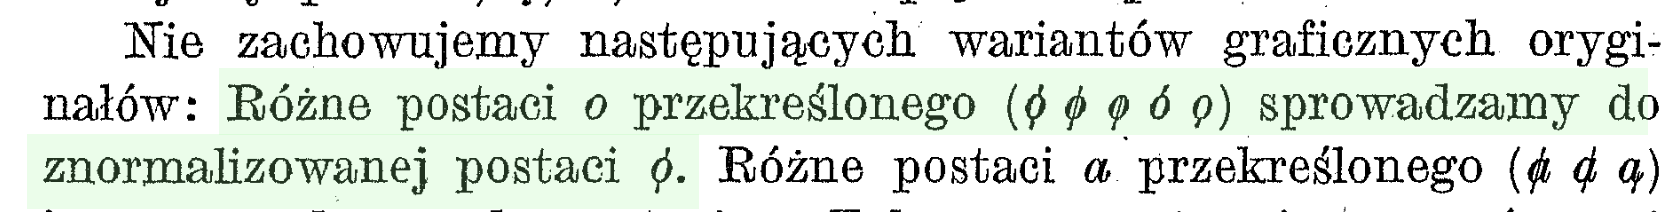
\includegraphics[width=0.95\hsize]{img/01_Zasady28-15orogate}

\caption{\textit{Zasady wydawania tekstów staropolskich} [\cite{Górski_Konrad__Zasady}] s. 28}
%\textit{O} przekreślone w ,,Zasadach \ldots''}
\label{fig:orogate}
\end{figure}


Cytowana na ilustracji reguła stosowania ,,o rogatego'' jest
praktycznie niewykonalna, ponieważ znak taki nie występuje we
współczesnych fontach --- mówiąc ściślej, występuje w fontach TeX Gyre,
% por. http: //www.gust.org.pl/tex-gyre na pozycjach ???,
ale niemal nikt o tym nie wie (np. nie wspomina się o tym w artykule
[\cite{boguslaw_jackowski_piotr_pianowski_piotr_strzelczyk_kolekcja_2018}]),
a jego użycie jest kłopotliwe\footnote{Od maja 2020 r. znak jest
  dostępny również w foncie JuniusX, patrz
  \url{https://github.com/psb1558/Junicode-New/issues/3} [uwaga dodana
  we wrześniu 2020~r.].}.

% ! Zgodnie bowiem z zale-
% ceniem zawartym w specyfikacji
% Unicode Standard
% [14] najpierw powinny być prze-
% twarzane akcenty dolne
%  Unicode Consortium,
% The Unicode Standard 10.0.0; chapter 3.11 Normalization Forms
% ;
% http://unicode.org/versions/Unicode10.0.0/ch03.pdf
% [dostęp 12.11.2018].


W artykule przedstawiam standard Unicode z perspektywy wykorzystania
go do kodowania polskich tekstów dawnych, jest to więc w pewnym
stopniu uzupełnienie artykułu [\cite{Strzelczyk_2013}], a w pewnym
stopniu również niejawna polemika z niektórymi jego tezami. Jest to
również uzupełnienie artykułu [\cite{bien_parkoszPSP}], gdzie pisałem:
\textit{Zasadniczym celem artykułu jest prezentacja założeń
  przygotowanej przeze mnie eksperymentalnej edycji
  elektronicznej, ma on jednak również ważny cel poboczny, mianowicie
  zainteresowanie Czytelników funkcjonowaniem konsorcjum Unicode,
  które ustala sposoby reprezentowania znaków w komputerach; dodanie
  znaków przydatnych dla dawnej polszczyzny do standardu  jest trudne,
  ale nie niemożliwe – wymaga jednak nie tylko wiedzy
  specjalistycznej, ale i orientacji w organizacji działalności
  normalizacyjnej} ([\cite[s. 27]{bien_parkoszPSP}].)

Prezentacja standardu z konieczności będzie mocno uproszczona
--- jak pisze Korpela [\cite*[s. 198 ]{korpela_unicode_2006}], podstawowe
zasady i struktura standardu są proste, ale Unicode jako całość jest
skomplikowany i zawiera trudne pojęcia, definicje i algorytmy.


Warto dodać, że konsorcjum Unicode utrzymuje również ,,wspólne
repozytorium danych lokalizacyjnych'' (\textit{Common Locale Data
  Repository}) zawierające informacje specyficzne dla konkretnych
języków, jak repertuar znaków, kolejność alfabetyczna itp. Wydaje się
celowe stworzenie odpowiedniego zestawu informacji dla dawnej
polszczyzny, ale to jest odrębny temat.

\section{Geneza standardu Unicode}
\label{sec:geneza-stand-unic}

Pierwsze komputery posiadały jako urządzenia wejścia/wyjścia sprzęt
korzystający z już istniejących nośników, jak taśma perforowana
(dalekopisy) lub karty perforowane, i stosowały zestawy znaków
zaprojektowane dla tych nośników, początkowo 6- i 7-bitowe, potem
także 8-bitowe. W epoce komputerów osobistych dominowały już kody
8-bitowe. Były one ograniczone do 256 znaków, co było często
niewystarczające, zwłaszcza dla tekstów wielojęzycznych. W związku z
tym opracowano koncepcję ,,rozszerzania kodu'', a ściślej jego zmiany
ograniczonej do wskazanego fragmentu tekstu; koncepcja została
sformalizowana w obszernym i skomplikowanym dokumencie przygotowanym
przez \textit{European Computer Manufacturers Association} jako
standard ECMA-35, a lepiej znanym jako norma ISO/IEC 2022
([\cite{wiki:ISO2022:2020}]).

% https://en.wikipedia.org/wiki/ISO/IEC_2022

Jest to ,,kodowanie stanowe'' (\textit{stateful encoding}) --- aby
zinterpretować fragment tekstu niezbędne jest przeczytanie go od
samego początku w celu odnalezienia kodów sygnalizujących właściwy
sposób interpretacji.

% https://nablux.net/tgp/weblog/2013/03/22/how-typeset-japanese-using-xelatex/
% fc-search-codepoint

% fonts-takao-mincho

%    Wednesday (10:45-12:05)
% Chair: Peter Honeyman

%     Hello World
%         Rob Pike & Ken Thompson, AT&T Bell Laboratories 


% http://doc.cat-v.org/plan_9/4th_edition/papers/utf

%  Hello World

% or

% Καλημέρα κόσμε

% or
% {\setmainfont{TakaoMincho} こんにちは 世界}
% {\fontspec{TakaoMincho} こんにちは 世界}
% こんにちは 世界
% Rob Pike
% Ken Thompson
% AT&T Bell Laboratories
% Murray Hill, New Jersey 07974

% The standard defines a sparse set of 32-bit characters, which would be
% hard to implement and have punitive storage requirements. Also, the
% standard attempts to mollify national interests by allocating 16-bit
% subspaces to national committees to partition individually. The sug-
% gested mode of use is to ‘‘flip’’ between separate national standards
% to implement the international stan- dard. This did not strike us as a
% sound basis for a character set. As well, transmitting 32-bit values
% in a
% byte stream, such as in pipes, would be expensive and hard to implement.

Było oczywiste, że należy zwiększyć liczbę bitów przeznaczonych na
reprezentację znaku. Radykalna propozycja wykorzystania 4 bajtów na 1
znak została sformułowana pod egidą Międzynarodowej Organizacji
Standaryzacyjnej ISO (razem z IEC --- Międzynarodowa Komisją
Elektrotechniczną --- firmującej m.in. wspomnianą normę ISO/IEC 2022),
zrzeszającej krajowe organizacje normalizacyjne z prawie wszystkich
państw świata. Według [\cite{Pike93}] pula dostępnych kodów miała być po prostu
rozdzielona między kraje członkowskie do wykorzystania według własnego
uznania. W dodatku nie zrezygnowano całkowicie z kodowania stanowego
(patrz także  [\cite{wiki:ISO10646:2020}]).

Było to rozwiązanie wysoce niepraktyczne z punktu widzenia producentów
oprogramowania, którzy przejęli inicjatywę i przygotowali projekt
standardu Unicode, przeznaczającego 16 bitów na znak reprezentowany
zawsze bezstanowo --- tekst można poprawnie interpretować
rozpoczynając czytanie w dowolnym miejscu. ISO ustąpiło i ustanowiona
w 1993 r. norma ISO/IEC 10646-1 \textit{Information technology --
  Universal Coded Character Set (UCS)} miała repertuar znaków i
podstawowe zasady zgodne ze standardem Unicode 1.1, w dodatku
postanowiono repertuar znaków synchronizować systematycznie (zdarza
się jednak, że znaki wprowadzone do repertuaru przez ISO są przez
Unicode niezalecane).  Dwa bajty na znak okazały się szybko
niewystarczające, począwszy od wersji 2.0 Unicode wykorzystuje
jednostki 21-bitowe (patrz np. [\cite{Blewitt16}]).
% A brief history of Unicode.pdf
% http://www.docklandsljc.uk/presentations/2016/AlexBlewitt-BriefHistoryOfUnicode.pdf
% https://www.infoq.com/presentations/unicode-history/ nagranie!!!
% https://play.google.com/store/apps/details?id=com.infoq.videos

Warto pamiętać, że w szczegółach norma ISO (aktualnie ISO/IEC
10646:2017 z późniejszymi dodatkami) cały czas różni się od standardu
Unicode (aktualnie wersja 12.1 z 7 maja 2019 r. definiująca 137 929
znaków\footnote{Zastapiona 10 marca 2020~r. przez wersję 13.0.0
  definiującą 143 859 znaków [uwaga dodana we wrześniu 2020~r.].}),
nie będziemy jednak się tym tutaj zajmować.

Aby ułatwić powszechną akceptację standardu Unicode, jego twórcy
zapewnili pełną zgodność repertuaru z pewną liczbą popularnych
zestawów znaków; te odziedziczone po wcześniejszych standardach znaki
są do dzisiaj źródłem różnych niekonsekwencji.

Podstawowym założeniem standardu jest reprezentowanie abstrakcyjnych
znaków, a nie ich kształtów czyli glifów. Abstrakcyjny znak może mieć
wiele kształtów, co jest raczej oczywiste, ale przyjmuje się również,
że konkretny glif może reprezentować różne abstrakcyjne znaki, co jest
już w dużym stopniu kwestią umowną.

Jednym z twórców standardu był Joseph D. Becker, który w swoim
artykule \textit{Multilingual Word Processing} z 1984 r. rozróżnił
wprowadzanie (\textit{input}), reprezentowanie
(\textit{reprezentation}) i zobrazowanie (\textit{rendering}) tekstu
([\cite{Becker1984}]).
% sprawdzić!
Problem w tym, że te 3 aspekty są do dziś przez wielu traktowane jako
jedyne możliwe sukcesywne etapy przetwarzania tekstu --- konsekwencją
tego jest silna tendencja do minimalizacji liczby znaków i zakładania,
że obsługa wariantów graficznych jest zadaniem autorów fontów. Ta
postawa była zrozumiała ćwierć wieków temu, ale w czasach masowej
dygitalizacji potrzebujemy często reprezentować wskanowany tekst jako
ciąg znaków zanim dokonamy jego ostatecznej interpretacji.

Istnieją też zastosowania, takie jak badanie proweniencji starych
druków, dla których właśnie glify są najbardziej istotne.  Ciekawą
inicjatywą wykorzystania do tego celu metod komputerowych był projekt
\textit{Cassetin} ([\cite{Cassetin2003}]) i późniejsze prace, np.
[\cite{andre:halshs-00983575}], które chyba nie są jednak
kontynuowane.
% https://tug.org/TUGboat/tb24-3/andre.pdf
%
%
Również trenowanie programów automatycznego rozpoznawania znaków ma
podobne potrzeby i wymaga specjalistycznych narzędzi. Odpowiedzialne
za standard konsorcjum Unicode ciągle ignoruje te potrzeby, ale mimo
tego dla standardu Unicode nie ma  alternatywy.

\section{Znaki Unicode}
\label{sec:znaki-unicode-i}

% \subsection{Klasyfikacja}
% \label{sec:klasyfikacja}



Jak było wspomniane, standard wykorzystuje jednostki
21-bitowe. Wszystkie liczby dające się w ten sposób reprezentować
stanowią \textit{przestrzeń kodową}, postrzeganą jako 17 płaszczyzn, z
których każda ma 256 wierszy w 256 kolumnach. Konkretna liczba to
\textit{punkt kodowy} (stosowałem również termin \textit{współrzędna
  kodowa}), w skrócie \textit{kod} --- tego użycia nie należy mylić ze
znaczeniem konkretnego zestawu znaków kodowych. Punkty kodowe
zapisujemy w postaci liczby heksadecymalnej poprzedzonej prefiksem
\textit{U+}, np. \ucode{U+754C}. Interesujące nas punkty kodowe są
również nazywane \textit{skalarami}\footnote{Skalarami nie są
  m.in. wspomniane niżej surogaty, którymi nie będziemy się w ogóle
  zajmować.}.

% https://en.wikipedia.org/wiki/Plane_(Unicode)


Standard wyróżnia 7 równorzędnych typów punktów kodowych, które tutaj
połączymy w bardziej intuicyjne grupy stosując własną terminologię;
\begin{itemize}
\item znaki ustalone (\textit{Graphic}, \textit{Format}, \textit{Control}),
\item znaki prywatne (\textit{Private-use}),
\item znaki specjalne (\textit{Surrogate},
  \textit{Noncharacter})
\item znaki rezerwowe (\textit{Reserved})
\end{itemize}
% Graphic, Format, Control, Private-Use, Surrogate, Noncharacter, Reserved

Znaki ustalone są zdefiniowane w standardzie w sposób stabilny --- ich
podstawowe własności nigdy nie będą zmienione. Znaki prywatne, jak
sama nazwa wskazuje, mają znaczenie i własności uzgodnione przez
zainteresowanych użytkowników w sposób niezależny od standardu.

% https://core.ac.uk/download/pdf/11337735.pdf
% http://www.postscriptum.us.edu.pl/pl/domowa/numery-archiwalne/1998-1999-27-29/

Z wcześniejszych standardów kodowania tekstów
(por. np. [\cite{bc286}]) standard Unicode przejął definicję znaku
(abstrakcyjnego), której tłumaczenie cytuję tutaj za [\cite{bc114}]:
% Definicja D3 (\cite{U4.0}, s.~64) określa to pojęcie następująco:
% \begin{quote}
%   A unit of information used for the organization, control, or representation of textual data
\textit{Jednostka informacji stosowana do organizacji danych tekstowych,
  sterowania nimi lub ich reprezentacji.}
% \end{quote}

% /mnt/MyBookT2/Bachotek04_Unicode/nowy
% Standard Unicode 4.0.\\ Wybrane pojęcia i terminy

% The smallest component of written language that has semantic value;
% refers to the abstract meaning and/or shape, rather than a specific
% shape (see also glyph), though in code tables some form of visual
% representation is essential for the reader’s understanding.

Oczywiście definicja taka jest pozbawiona praktycznego znaczenia,
dlatego wolę inną definicję sformułowaną w cytowanym wyżej artykule
(tutaj przytaczam ją nieznacznie zmodyfikowaną): \textit{znak Unicodu
  to pojęcie pierwotne, zdefiniowane przez wyliczenie}.

% https://en.wikipedia.org/wiki/Unicode_character_property

Wyliczenie to polega na mniej lub bardziej jawnym wyliczeniu własności
przypisanych do danego punktu kodowego. Najważniejszą własnością jest
umowna \textit{nazwa}, np. \uname{LATIN SMALL LETTER A WITH OGONEK};
standard gwarantuje, że nigdy ona nie ulegnie zmianie, nawet gdy jest
w jakimś sensie niepoprawna; punktowi kodowemu może być jednak
przypisany w razie potrzeby \textit{alias}.

% Unicode Technical Note #27
% Known Anomalies in
% Unicode Character Names
% http://www.unicode.org/notes/tn27/tn27-4.html

Drugą ważną własnością znaków jest ich \textit{kategoria}
(ang. \textit{general category}), np. \textit{Lc} oznacza literę w kaszcie
górnej. Wszystkich możliwych wartości jest 29.

Prawdopodobnie pierwotne ograniczenie do 16 bitów leży u podstaw
zasady, że diakryty są w zasadzie kodowane jako oddzielne
\textit{znaki dostawne} (ang. \textit{combining characters}) dodawane
do \textit{znaków bazowych} (ang. \textit{base characters}). Wszystkie
znaki dostawne mają kategorię \textit{Mn} (ang. \textit{Mark,
  non-spacing}). Sposób, w jaki znak dostawny łączy się ze znakiem
bazowym, jest określony przez własność \textit{łączliwość}
(ang. \textit{Combine}) --- na przykład znak \uname{COMBINING
  OGONEK} % (U+0328)
ma łączliwość równą 202, co oznacza \textit{Attached Below}.

Znaki dostawne są zapisywane zawsze po znaku bazowym, ich kolejność ma
znaczenie tylko wtedy, gdy na siebie oddziałują graficznie --- znak
występujący wcześniej powinien być zobrazowany bliżej znaku bazowego
niż znak występujący później. Standard nie nakłada żadnych ograniczeń
na liczbę znaków dostawnych odnoszących się do jednego znaku bazowego,
co pozwala dla zabawy tworzyć tzw. teksty Zalgo\footnote{Więcej na ten
  temat pod adresem \url{https://zalgo.org/}.}. Sekwencję znaków
zapisujemy w nawiasach kątowych oddzielając je przecinkami,
np. \ucode{<U+012F, U+0307, U+0301}>; sekwencje mogą mieć swoje nazwy,
np. przytoczona sekwencja nazywa się \uname{LATIN SMALL LETTER I WITH
  OGONEK AND DOT ABOVE AND ACUTE} (podobno stosowana w języku
litewskim w specjalistycznych publikacjach).
% lotewski???: !!!LATIN CAPITAL LETTER A WITH OGONEK AND ACUTE;0104 0301
% combing with class 0

% /home/jsbien/UnicodeDemistyfied/read.pudn.com/downloads121/ebook/513123/Unicode.Demystified.pdf

% All non-combining characters have a combining class of 0. A fair
% number of combining marks also have a combining class of 0, which
% indicates that the mark combines typographically with its base
% character in a way that should prevent reordering of any marks
% attached to the same character. For example, the enclosing marks have
% a combining class of 0.

% Mark (M): spacing combining (Mc), enclosing (Me), non-spacing (Mn)

% % https://en.wikipedia.org/wiki/Combining_character

% % https://en.wikipedia.org/wiki/Combining_Grapheme_Joiner

% % https://en.wikipedia.org/wiki/Zero-width_non-joiner


% % https://en.wikipedia.org/wiki/German_keyboard_layout

% łączliwość


% własności
% normatywne 
% informacyjne
% wtórne

Na potrzeby segmentacji tekstu na słowa i na ,,znaki postrzegalne''
(ang. \textit{user-perceived characters}) w wersji 3 standardu
pojawiło się pojęcie \textit{zbitki grafemicznej} (\textit{graphemic
  cluster}), a potem pojęcie \textit{rozszerzonej zbitki grafemicznej}
(\textit{extended graphemic cluster}). Przykłady ilustrujące te
pojęcia w normatywnym aneksie do standardu nr 29 pochodzą głównie z
pisma koreańskiego, tajskiego i dewanagari; z pisma łacińskiego
pochodzi przykład sekwencji \textit{ch}, której w niektórych językach
odpowiada w wymowie jedna spółgłoska --- w konsekwencji zapis ten może
być uznany za jeden grafem, ale jest moim zdaniem dyskusyjne, czy jest
to jeden ,,znak postrzegalny''. Nie ulega jednak wątpliwości, że dla
zwykłego użytkownika pojęcie rozszerzonej zbitki grafemicznej jest
bliższe intuicyjnemu rozumieniu znaku piśmiennego niż pojęcie
abstrakcyjnego znaku zdefiniowane w standardzie.

Zasada reprezentowania tylko abstrakcyjnych znaków, a nie ich
kształtów, została naruszona przez wprowadzenie w wersji 3.2
selektorów wariantów (\textit{variant selector}). Teoretycznie ich
zakres użycia jest bardzo szeroki --- por. stwierdzenie
\footnote{\url{https://www.unicode.org/faq/vs.html\#18},
  także \url{https://bit.ly/2CjcsVA-vsUnicode}.}:
\begin{quote}
  Dla historycznych systemów pisma sekwencje wariacyjne są
  pożytecznym narzędziem, ponieważ pozwalają zakodować błędne lub
  rzadkie (ang. \textit{nonce}) czcionki (ang. \textit{glyphs}) w
  sposób ukazujący ich związek ze znakiem podstawowym.
\end{quote}
Praktyka jest jednak bardzo restryktywna ---
por. np. \cite{wiki:Vforms:2020}, [\cite{wiki:VS:2020}];
% https://en.wikipedia.org/wiki/Variation_Selectors_(Unicode_block)
co najmniej jedna propozycja użycia selektorów wariantów została
odrzucona z nieznanych mi
powodów\footnote{Por.
  \url{https://www.unicode.org/mail-arch/unicode-ml/y2018-m07/0120.html}.}.

% \url{http://www.unicode.org/mail-arch/unicode-ml/y2010-m08/0020.html}
% From: Janusz S. Bień via Unicode <unicode_at_unicode.org>
% Date: Mon, 30 Jul 2018 06:41:00 +0200

% On Mon, Jul 16 2018 at 7:07 +0200, jsbien_at_mimuw.edu.pl writes:

% [...]

% > To the best of my knowledge, the only attempt to introduce additional
% > variation sequences was the strongly criticised Karl Pentzlin's proposal
% > L2-11/059
% >
% > http://www.unicode.org/L2/L2011/11059-latin-cyr-var.pdf
% >
% > What has happen to it? I don't remember any information about it on the
% > list.

% Anybody willing to share his knowledge on this topic?

% Looking for something else I found

% L2/13‐153

% Proposal to Use Standardized Variation Sequences to Encode Church
% Slavonic Glyph Variants in Unicode
% https://www.unicode.org/L2/L2013/13153-variants.pdf

% I don't remember the proposal being discussed on the list and I was
% unable to find any trace of a discussion in the list archives. Is my memory
% correct?

% I found also

% L2/13‐164
% Expert Feedback on Cyrillic proposals...
% https://www.unicode.org/L2/L2013/13164-cyrillic-fdbk.pdf

% containing interesting comments on VS by David Birnbaum.

% I understand L2/13‐153 and L2/13-153 has been rejected, but I would be
% happy to have more information about it.

% Best regards 
{\tolerance 900 Aktualny wykaz zatwierdzonych wariantów znajduje się w
  Bazie Znaków Unicode (patrz punkt \vref{sec:forma-stand-unic}) w
  pliku {\relsize{-1}\texttt{StandardizedVariants.txt}}; ponad 1000
  pozycji dotyczy sinogramów (ang. i jap. \textit{kanji} --- znaków
  powstałych na początku naszej ery w Chinach za panowania dynastii
  Han), ponad 200 dotyczy tzw. emoji, około 30 znaków matematycznych,
  pozostałe dotyczą języka mongolskiego. Ze względu na szerokie
  zastosowania sinogramów, używanych w Chinach i Japonii, a wcześniej
  również w Korei i Wietnamie, i wynikające z tego bardzo różnorodne
  potrzeby użytkowników, konsorcjum Unicode utrzymuje dodatkowo bazę
  \textit{Ideographic Variation Database}, gdzie można rejestrować
  zgodnie z odpowiednią procedurą alternatywne kolekcje wariantów
  sinogramów (aktualnie baza liczy około 40 tysięcy pozycji).

  Obsługa selektorów wariantów jest uwzględniona w specyfikacji fontów
  komputerowych OpenType w postaci osobnej podtablicy (typu 14)
  tablicy odwzorowania \texttt{cmap},
  por. np. [\cite{microsoft:_charac_glyph_index_mappin_table}].

}
W zasadzie diakryty (znaki dostawne) odnoszą się zawsze do jednego
znaku bazowego, wyjątkowo do dwóch, np.  \uname{COMBINING DOUBLE
  TILDE}. Zasada ta w pewnym sensie została naruszona przez
wprowadzenie znaków \uname{COMBINING CYRILLIC TITLO LEFT HALF} i
\uname{COMBINING CYRILLIC TITLO RIGHT HALF}
[\cite{titlo2013}]\footnote{Dla pełności obrazu można też wspomnieć
  o niezalecanych znakach adnotacji interlinearnych
  (\ucode{U+FFF9}--\ucode{U+FFFB}).}.



% Jednak według s. 125 demystyfying diakryty mogą się
% odnosić do całej zbitki grafemicznej.

% demystified  
% A non-spacing mark applies to all characters up to the nearest preceding grapheme cluster boundary,
% provided they're not a conventional combining character sequence (if they are, the non-spacing mark is just
% part of that combining character sequence). This rule mainly states that non-spacing marks following
% Hangul syllables apply to the whole syllable, regardless of how it's represented.

% { \fontspec{FreeMono} 
% 1͏2⃝
% }  
%   joiner

%   https://www.w3.org/TR/unicode-xml/#Interlinear

Przestawione zasady powodują występowanie zapisów równoważnych. Typowy
przykład to znak samodzielny, odziedziczony po jakimś wcześniejszym
kodzie jak \uname{LATIN SMALL LETTER A WITH OGONEK}, i zapis w formie
sekwencji zestawionej ze znaków \uname{LATIN SMALL LETTER A} i
\uname{COMBINING OGONEK}.  Jeśli znaki diakrytyczne nie oddziałują
na siebie (np. jeden jest nad znakiem, a drugi pod nim), to ich
kolejność w sekwencji zestawionej jest obojętna. W rezultacie
sprawdzenie, czy dwa napisy --- czyli sekwencje punktów kodowych ---
są równe, wymaga ich \textit{normalizacji}, co jest dla programisty
błędogenną komplikacją. W dodatku dwa typy normalizacji zdefiniowane w
standardzie --- kanoniczna i dostosowawcza
(ang. \textit{compatibility}) --- nie zawsze odpowiadają potrzebom
użytkownika, co zilustrujemy później.

\section{Forma standardu Unicode}
\label{sec:forma-stand-unic}

Podstawową formą standardu jest \textit{Baza Znaków Unicode}
(ang. \textit{Unicode Character Database}, w skrócie UCD).  Baza
dostępna jest w wersji XML, ale bardziej praktyczna jest wersja czysto
tekstowa ze względu na mniejszą objętość. Składa się z pewnej liczby
plików, z których najważniejszy jest \texttt{UnicodeData.txt}. Oto
przykład jednego wiersza tego pliku (dla przejrzystości podzielonego
tutaj na fragmenty):

{%\relsize{-2}
\begin{verbatim}
0105;LATIN SMALL LETTER A WITH OGONEK;
Ll;0;L;0061 0328;;;;N;
LATIN SMALL LETTER A OGONEK;;
0104;;0104
\end{verbatim}
}

Na początku wiersza mamy punkt kodowy, potem oddzielone średnikami
m.in. następujące własności: nazwa, kategoria (Ll --- litera z dolnej
kaszty), rozkładalność na sekwencję <U+0061,U+0328>, przestarzała
nazwa stosowana w Unicode 1.0, odpowiednik w kaszcie górnej i
tzw. tytułowej (U+0104).

% http://www.unicode.org/reports/tr44/
% Ken Whistler (ken@unicode.org) and Laurențiu Iancu (liancu@unicode.org)
% Unicode® Standard Annex #44
% Unicode Character Database

% [UTR23] 	Unicode Technical Report #23: The Unicode Character Property Model

Inny przykład, to fragment pliku \texttt{NamedSequences.txt}:
\begin{quote}
\begin{verbatim}
# Additions for Lithuanian.
# Provisional 2006-05-18, Approved 2007-10-19
LATIN CAPITAL LETTER A WITH OGONEK AND ACUTE;0104 0301
\end{verbatim}
\end{quote}
Oczywiście baza ta nie jest przeznaczona do bezpośredniego
wykorzystania przez człowieka. Do przeglądania jej zawartości w
wygodny sposób zostały stworzone różne narzędzia.  Nie jest to
właściwe miejsce na dokonanie ich przeglądu, wspomnę tylko o
kilku. Witryna Unicode oferuje wyszukiwarkę różnych własności i pokaz
działania wybranych algorytmów pod adresem
\url{https://unicode.org/cldr/utility}.  Do lokalnej instalacji
przeznaczony jest program \textsf{Unibook™ Character Browser}
(\url{https://unicode.org/unibook/help/unibook.htm}), dostępny
niestety tylko dla MS Windows, wprawdzie bezpłatny, ale o zamkniętym
kodzie --- firmuje go Asmus Freytag, jeden z twórców standardu. Z
narzędzi online godna polecenia jest witryna
\url{https://codepoints.net/}, do której jeszcze wrócimy.
% Do narzędzi tych jeszcze
% powrócę dalej.

Druga część standardu to tabele kodów z przykładowymi glifami,
pochodzącymi z różnych także komercyjnych fontów --- są one
przygotowywane za pomocą wspomnianego wyżej programu \textsf{Unibook}
na podstawie pliku \texttt{NamesList.txt}, który również należy do
UCD. Oto przykładowy fragment:

\begin{quote}
\begin{verbatim}
0104	LATIN CAPITAL LETTER A WITH OGONEK
	: 0041 0328
0105	LATIN SMALL LETTER A WITH OGONEK
	* Polish, Lithuanian, ...
	: 0061 0328
\end{verbatim}
\end{quote}

Fragment ten zawiera informacje o dekompozycji kanonicznej
(objaśnionej dalej) i niekonsekwentne komentarze (chyba odziedziczone po
standardach ISO), plik zawiera też inne informacje umieszczane w tabeli
kodów.

Trzecia część to opis standardu w języku angielskim w formie plików
PDF; opis zawsze dotyczy aktualnej wersji, z nielicznymi wyjątkami nie
zawiera informacji historycznych, w szczególności nie podaje
informacji o motywach uwzględnienia w standardzie konkretnych znaków
--- informacji takich należy szukać za pośrednictwem \textit{Unicode®
  Technical Committee Document Registry}
(\url{https://unicode.org/L2/}). Zarówno tabele, jak i opis jest
dostępny bezpłatnie na witrynie konsorcjum Unicode; wersje papierowe
mogą być do nabycia na zasadzie druku na żądanie.

Postać stosowanych w standardzie tabel kodów jest wygodna i
przejrzysta, dlatego Ievgenii Meshcheriakov stworzył program
\textsf{fntsample}, który w tym formacie produkuje tabele dla
wskazanego fontu lub jego fragmentu --- program, na otwartej licencji,
jest aktualnie dostępny pod adresem
\url{https://github.com/eugmes/fntsample}. Jeden z moich studentów,
Paweł Parafiński, w 2013 r. na moją prośbę stworzył rozszerzenie tego
programu upodabniające wyniki jeszcze bardziej do tabel standardu
przez uzupełnienie tabel fontu o komentarze pochodzące z oryginalnego
pliku \texttt{NamesList.txt} lub z własnego pliku przygotowanego w tym
formacie. Rozszerzenie to znajduje się obecnie w dwóch repozytoriach
\url{https://bitbucket.org/jsbien/unicode-ucd-parser} i
\url{https://bitbucket.org/jsbien/fntsample-fork-with-ucd-comments}\footnote{Meshcheriakov
  rozważał włączenie tych funkcji do swojego programu, ale dotąd to
  nie nastąpiło ---
  por. \url{https://github.com/eugmes/fntsample/issues/7}/}.
% Przykład
% użycia można znaleźć w repozytoriach, o których będzie mowa później.

Twórcą i administratorem wspomnianej wcześniej witryny
\url{https://codepoints.net/} jest Manuel Strehl. Wyróżnia się ona od
innych podobnych witryn m.in. tym, że w pewnym sensie je integruje:
strona dla konkretnego znaku,
np. \url{https://codepoints.net/U+A76B?lang=en}, zawiera linki między
innymi do stron
\url{https://unicode.org/cldr/utility/character.jsp?a=A76B},
\url{https://fileformat.info/info/unicode/char/A76B/index.htm},
\url{https://graphemica.com/ꝫ},
\url{https://scriptsource.org/char/U00A76B} i
\url{https://www.isthisthingon.org/unicode/index.phtml?glyph=A76B}
(Unisearcher). Dodatkowy link %--- jeśli działa ---
pokazuje glif znaku wycięty z oryginalnej tabeli
standardu\footnote{%Haralambous %[\citeyear{haralambous02:_unicod}] nie linkuje!
  [\cite{haralambous02:_unicod}] nazywa go glifem uprzywilejowanym
  (fr. \textit{glyphe privilégié}), ja wolałbym chyba nazywać go
  glifem demonstracyjnym (ang. \textit{demonstrative}).}.
% glyph specimen  glif okazowy???

% Haralambous Yannis, « Unicode et typographie : un amour impossible »,
% Document numérique, 2002/3 (Vol. 6), p. 105-137. DOI :
% 10.3166/dn.6.3-4.105-137. URL :
% https://www.cairn.info/revue-document-numerique-2002-3-page-105.htm

Głównym atutem tej witryny są dla mnie linki do odpowiednich stron
Wikipedii. Choć w angielskiej wersji zdarzają się błędy (por. np. mój
wpis w dyskusji hasła \url{https://en.wikipedia.org/wiki/UTF-16}),
czasami zawierają one trudno dostępne informacje, a mianowicie linki
do dokumentów zawierających uzasadnienie włączenia danych znaków do
standardu. Dokumenty te są publicznie dostępne za pośrednictwem już
wspomnianego \textit{Unicode® Technical Committee Document Registry},
ale odnalezienie interesującego dokumentu bywa kłopotliwe. Wprawdzie
hasła Wikipedii nie zawsze podają odpowiednie linki w optymalny
sposób, wydaje się jednak, że wykorzystywanie jej do tego celu i
popieranie tej inicjatywy jest lepsze niż tworzenie jakiegoś
alternatywnego indeksu. Można w szczególności rozważyć stworzenie
specjalnego portalu
(por. \url{https://pl.wikipedia.org/wiki/Wikipedia:Portal}) lub
projektu
(por. \url{https://pl.wikipedia.org/wiki/Wikipedia:Wikiprojekt}).

% https://codepoints.net/U+A76B?lang=pl

Źródła witryny \url{https://codepoints.net/} są dostępne na swobodnej
licencji i utrzymywane za pomocą systemu zarządzania wersjami ---
patrz \url{https://github.com/Codepoints/codepoints.net}. Język
interfejsu jest modyfikowalny, ponieważ wszystkie napisy są zapisane
zgodnie z konwencją \textit{gettext}
(por. np. \url{https://pl.wikipedia.org/wiki/GNU_gettext}). W dodatku
autor zapewnił dostęp do witryny wspomagającej tłumaczenie
(\url{https://crowdin.com/project/codepoints}).

Wszystko to sprawiło, że w 2016 r. podjąłem próbę polonizacji tej
witryny (nieco pomogła mi w tym Joanna Bilińska). Wynik jest dostępny,
ale nie jest to wersja kompletna i ostateczna --- prace nad
polonizacją z różnych względów zaniechałem, ale byłoby dobrze, gdyby
ktoś je kontynuował.

Jeśli tylko jest to możliwe, polskojęzyczna wersja witryny kieruje ---
co jest w zasadzie słuszne --- do polskojęzycznej wersji
Wikipedii. Niestety polskie hasła dotyczące znaków standardu nie tylko
są mniej liczne i uboższe treściowo, ale i mniej wiarygodne. Edycja
haseł Wikipedii wymaga nie tylko wiedzy, ale i talentów
dyplomatycznych oraz cierpliwości w dyskusjach z innymi wikipedystami,
którym się wydaje, że wiedzą wszystko lepiej\ldots Pomimo tego warto
podejmować próby doprowadzenia polskich haseł dotyczących standardu do
satysfakcjonującego poziomu.

% https://github.com/Codepoints/Codepoints.net/issues/74
% https://github.com/Codepoints/codepoints.net

% https://pl.wikipedia.org/wiki/GNU_gettext


\section{Znaki prywatne}
\label{sec:znaki-prywatne}

Na znaki prywatne przeznaczone są trzy obszary: 6 400 punktów kodowych
na Podstawowej Płaszczyźnie Wielojęzycznej (BMP) i praktycznie całe
płaszczyzny nr 15 i 16 po 65 534 punktów każda (ze względu na wysokie
wartości kodów korzystanie z tych płaszczyzn jest mniej wygodne niż z
BMP).

Ponieważ nie ma obowiązku rejestrowania porozumień dotyczących
wykorzystania znaków prywatnych, sporządzenie ich pełnego wykazu jest
niemożliwe. Pewną liczbę przykładów podaje artykuł [\cite{wiki:PUA:2020}].
Najczęstszym motywem korzystania ze znaków prywatnych jest
niedostępność w standardzie potrzebnego znaku, odpowiedniej sekwencji
dostawnej lub zbitki grafemicznej. Są też powody czysto techniczne
używania znaków prywatnych, które dają się reprezentować w standardzie
jako sekwencje dostawne --- pozwala to tworzyć fonty, w których
kształt i położenie diakrytów są dopracowane indywidualnie dla
konkretnego znaku, a nie są konsekwencją ogólnych algorytmów.

% Haugen Odd Einar, « Dealing with glyphs and characters. Challenges in
% encoding medieval scripts », Document numérique, 2013/3 (Vol. 16),
% p. 97-111. DOI : 10.3166/DN.16.3.97-111. URL :
% https://www.cairn.info/revue-document-numerique-2013-3-page-97.htm

Jednym z przykładów wykorzystania znaków prywatnych są ustalenia
inicjatywy stworzenia fontów unikodowych dla tekstów średniowiecznych
(\textit{Medieval Unicode Font Initiative}, w skrócie MUFI --- patrz
[\cite{einar13:_dealin}] i \url{https://mufi.info/}.
% \goodbreak
Od 2001 r. ukazały się 4 wersje rekomendacji, ostatnia w 2015
r. [\cite{haugen15:_mufi}]; inicjatywa ta wydaje się niestety martwa
--- chyba uznano, że cele zostały osiągnięte\footnote{Jak się okazuje,
  stwierdzenie to było zbyt pesymistyczne. Niedostępna przez dłuższy
  czas witryna projektu wróciła na swój pierwotny adres, ale aktualna
  rekomendacja jest dostępna tylko w formie elektronicznej ---
  por. np.
  \url{https://mufi.info/m.php?p=mufiversion&v=Characters added after v. 4.0}.
  [Uwaga dodana we wrześniu 2020 r.]}. Wersja 4 uwzględnia postulowaną
przeze mnie ligaturę długiego \textit{s} i małego \textit{ł}
występującą w korpusie IMPACT [\cite{bc381}] (aktualnie używany jest
kod przyjęty w stworzonej \textit{ad hoc} na potrzeby projektu
modyfikacji fontu \textit{DejaVu Sans} ---
por. \url{http://dl.psnc.pl/activities/projekty/impact/results/}). Uwzględnienie
znaku w specyfikacji MUFI daje nadzieję, że znak ten pojawi się
również w innych fontach, choć na dzisiaj jedynym fontem zgodnym z
najnowszą wersją specyfikacji jest \textit{Junicode} w wersji 1 lub
wyższej (\url{http://junicode.sourceforge.net/}), dostępny na otwartej
licencji\footnote{Od lipca 2020 r. znak dostępny również w fontach
  Kurinto Font Folio
  (\url{https://github.com/ClintGoss/Kurinto/issues/6}) [Uwaga dodana we wrześniu 2020 r.]}.

Wszystkie wersje specyfikacji mają postać ręcznie opracowanych tekstów
w formacie PDF, co nie ułatwia automatycznego przetwarzania omawianych
w nich znaków. Wyszukiwarka dostępna na witrynie MUFI nie obsługuje
wersji 4\footnote{Dotyczy poprzedniej wersji witryny [Uwaga dodana we
  wrześniu 2020 r.].}, w dodatku ani oprogramowanie ani wykorzystywane
dane nie są udostępnione w wersji źródłowej. W tej sytuacji na duże
uznanie zasługuje Rebecca G. Bettencourt, która we własnym zakresie
stworzyła pliki w formacie \texttt{UnicodeData.txt} m.in. dla znaków
MUFI (\url{http://www.kreativekorp.com/charset/PUADATA/}.

W artykule [\cite{bc480}] zaproponowałem, aby kody znaków prywatnych
zgodnych z rekomendacją MUFI poprzedzać prefiksem \texttt{M+} zamiast
\texttt{U+}, na przykład kod wspomnianego na s. \pageref{virgula}
znaku \texttt{SMALL VIRGULA} możemy zapisać M+F1F7.

Dla pełności obrazu chciałbym również wspomnieć, że cenna moim zdaniem
inicjatywa, z którą w 2012 r. wystąpił Andreas Stötzner, pozostała
praktycznie bez echa --- informacje o niej są obecnie dostępne tylko w
archiwum Internetu (\url{https://bit.ly/2XVTzRL-LINCUA}); proponował on
koordynację wykorzystania PUA do szeroko rozumianych celów
lingwistycznych.


Wykorzystanie znaków prywatnych do składu dawnych tekstów polskich
jest moim zdaniem nieuniknione.

% https://en.wikipedia.org/wiki/Private_Use_Areas
% BMP (0) 	Private Use Area 	6,400

% PUP (15)[d] 	Supplemental Private Use Area-A 	65,534
% PUP (16)[d] 	Supplemental Private Use Area-B 	65,534 

% http://unicode.org/pipermail/unicode/2018-August/006903.html

% http://www.kreativekorp.com/charset/PUADATA/

% https://debbugs.gnu.org/cgi/bugreport.cgi?bug=32599
% https://groups.google.com/forum/#!msg/gnu.emacs.bug/SK-RO_OG_GQ/BmUzA-23AgAJ

% https://skaldic.abdn.ac.uk/m.php?p=mufi
% http://andron-typeforum.xobor.de/t10f13-Towards-a-linguistic-corporate-use-area-LINCUA.html

% https://web.archive.org/web/20170905163108/http://andron-typeforum.xobor.de/t10f13-Towards-a-linguistic-corporate-use-area-LINCUA.html

% https://web.archive.org/web/20141105043327/http://andron-typeforum.xobor.de/file.php?url=http%3A%2F%2Ffiles.homepagemodules.de%2Fb578506%2
% Ff13t10p14n2.pdf&r=&content=Towards_a_linguistic_corporate_use_area%3F_%28LINCUA%29


% inicjatywa LINCUA (\textit{LINguistic Corporate Use Area}) którą w
% 2012 r. zaproponował Andreas Stötzner, też wygląda na martwą
% \footnote{Informacja o niej jest obecnie dostępna tylko w archiwum
% Internetu, patrz \url{http://bit.ly/2XVTzRL-LINCUA} [dostęp:
% 2019-05-10].}; szansą na jej ożywienie była propozycja, którą
% Stötzner złożył w lipcu 2018 r., włączenia się w ewentualne prace
% nad fontami dla dawnej polszczyzny\footnote{Patrz np.
% % \url{http://www.man.torun.pl/archives/arc/gust-l/2018-07/msg00003.html}
% \url{http://bit.ly/2CjNpBS-GUST} [dostęp: 2019-05-10] i
% \url{http://bit.y/2HvfsBL_DARIAH-PL} [dostęp: 2019-05-10].},
% która jednak nikogo nie zainteresowała.  Wadą tego podejścia jest
% to, że w celu umożliwienia wyświetlenia tekstu niezbędne jest nie
% tylko stworzenie odpowiedniego fontu, ale i dostarczenie go
% użytkownikowi.

% https://github.com/Codepoints/Codepoints.net/issues/106

\section{Tekstele}
\label{sec:tekstele}

Od dawna uważam, że aparat pojęciowy standardu Unicode jest
niewystarczający. Powstają w związku z tym dwa pytania: jakie
dodatkowe pojęcia zdefiniować i jak je nazwać.

Najbardziej potrzebne jest pojęcie, które odnosiłoby się do elementu
tekstu niezależnie od sposobu jego zapisu, np. obejmujące łącznie
\uname{LATIN SMALL LETTER A WITH OGONEK} i sekwencję \uname{LATIN
  SMALL LETTER A} i \uname{COMBINING OGONEK}. W standardzie jest
zdefiniowane pojęcie kanonicznej dekompozycji, oznaczane myląco
znakiem równoważności ({\fontspec{DejaVuMathTeXGyre-Regular}≡}) choć
nie jest to relacja symetryczna; np. sekwencja \uname{LATIN SMALL
  LETTER A} i \uname{COMBINING OGONEK} jest kanoniczną dekompozycją
\uname{LATIN SMALL LETTER A WITH OGONEK}, ale oczywiście nie
odwrotnie.  Jeśli dwa elementy tekstu mają taką samą kanoniczną
dekompozycję to są kanonicznie równoważne (ta relacja nie ma swojego
oznaczenia, choć jest równoważnością w matematycznym sensie). Pozornie
proponowane pojęcie mogłoby być zdefiniowane jako klasa abstrakcji dla
relacji kanonicznej równoważności, ale twórcy standardu skomplikowali
sprawę uznając, że relacja ta zachodzi między niektórymi pojedynczymi
znakami, np. \uname{OHM SIGN} i \uname{GREEK CAPITAL LETTER OMEGA};
znaki te wyglądają identycznie, ale niosą one inną informację, z
której użytkownik może nie chcieć rezygnować.

Bardzo przydatną metodą analizy tekstu jest sporządzenie histogramu
(wykazu częstości) znaków. Dla tekstów zapisanych zgodnie z standardem
Unicode do dzisiaj jedynym łatwo dostępnym (np. w dystrybucjach
systemu Linux) narzędziem jest program \textsf{unihist}, wchodzący w
skład zestawu narzędzi, których autorem jest Bill Poser (patrz
\url{https://www.billposer.org/Software/unidesc.html#unihist}); znaki dostawne są
zliczane osobno, co moim zdaniem czyni program mało przydatnym. W 2008
r. mój student Piotr Findeisen przygotował według mojej specyfikacji
program \textsf{unihistext}, który jest pozbawiony tej wady --- zlicza
obiekty o tej samej nazwie, a sekwencje mają nadane nazwy za pomocą
dostarczonego przez użytkownika pliku w formacie
\texttt{NamedSequenced.txt}, taki plik został przygotowany m.in. dla
prywatnych znaków MUFI. Obecnie program jest dostępny w repozytorium
\url{https://bitbucket.org/jsbien/unihistext/}, ale jest to niestety
program osierocony.

Obiekty, które zlicza program \textsf{unihistext}, są przykładem
obiektów, które proponuję nazywać \textit{tekstelami} --- powinny one
być definiowane przez wyliczenie, ponieważ trzeba nadać im nazwy
(niekoniecznie jawnie, mogą być tworzone za pomocą odpowiednich reguł
mniej lub bardziej mechanicznie). Tekstele mają też inne własności,
ale wynikają one w oczywisty sposób z własności ich znaków składowych.

Na składowe teksteli możemy mówić \textit{tekstony}, aby jawnie
odróżnić znak o kodzie \ucode{U+0105} od tekstela o nazwie
\uname{LATIN SMALL LETTER A WITH OGONEK} (można pomyśleć o jakiejś
odrębnej konwencji zapisywania nazw teksteli, ale na tym etapie to
chyba zbędna komplikacja).

Standard definiuje również odwzorowanie dostosowawcze, oznaczane
znakiem {\fontspec{DejaVuMathTeXGyre-Regular}≋}. Informuje ono, że
znaki lub ich sekwencje są w jakimś sensie podobne. Na przykład
ligatury są rozpisywane na składowe, np. znakowi \uname{LATIN SMALL
  LIGATURE FI} odpowiada sekwencja \uname{LATIN SMALL LETTER F} i
\uname{LATIN SMALL LETTER I}, co jest sensowne. Jednak niektóre inne
decyzje szczegółowe są kontrowersyjne, np. \uname{MICRO SIGN} ma
odwzorowanie dostosowawcze na \uname{GREEK SMALL LETTER MU} (dlaczego
nie kanoniczne?), a \uname{LATIN SMALL LETTER LONG S} na \uname{LATIN
  SMALL LETTER S}.  Przygotowując przeszukiwalną dygitalizację
\textit{Słownika polszczyzny XVI wieku}
[\cite{bien_dygitalizacja_2010}] chcieliśmy rozpisać ligatury
(użytkownik pisząc kwerendę nie powinien zajmować się kwestiami czysto
typograficznymi), ale zachować długie \textit{s}, które jest istotnym
elementem tekstów z tego okresu (w kwerendzie w razie potrzeby można
utożsamić długie i krótkie \textit{s} stosując wyrażenia regularne), w
konsekwencji nie mogliśmy użyć normalizacji dostosowaczej. Jest to
więc też zastosowanie pojęcia \textit{tekstela}, choć tym razem
niejawne.

Stosunkowo mało znany i względnie nowy język programowania Swift
definiuje znakowy typ danych następująco: \textit{Every instance of
  Swift’s Character type represents a single extended grapheme
  cluster.}\footnote{(\url{https://docs.swift.org/swift-book/LanguageGuide/StringsAndCharacters.html}.}.
Inny słowy podstawowym znakowym typem danych jest swoisty ,,znak
postrzegalny'', który moim zdaniem jednak zdecydowanie lepiej nazywać
\textit{tekstelem}.

%   Podejrzewam, że definicja ta nie oddaje w pełni
% własności tego typu danych --- tak czy inaczej, pokazuje to
% niezręczność oryginalnej terminologii standardu: każdy ,,znak
% postrzegalny'' to rozszerzona zbitka\ldots Moim zdaniem jest to
% dodatkowy argument za



% \printbibliography

% \end{document}

% Jak dotąd jeden tylko język programowania oferuje
%   rozszerzone zbitki grafemiczne jako osobny typ danych --- jest to
%   Swing\footnote{Patrz np. \textit{Every instance of Swift’s Character
%       type represents a single extended grapheme cluster.}
%     (\url{https://docs.swift.org/swift-book/LanguageGuide/StringsAndCharacters.html}).}.
%   $$\equiv$$ U+224b ≋ (≡

% ./stary_komputer/repliki/fleksem/grant/marasca.tex66:możemy nazywać w skrócie tekstelami (???).

% Na potrzeby wyszukiwania tekst jest traktowany jako ciąg napisów.
% Przez napis rozumiemy ciąg znaków w sensie omówionym wyżej, czyli ciąg
% teksteli. Napisy, na które został podzielony tekst, nazywamy krótko
% \textit{segmentami} (to termin powszechnie przyjęty) lub
% \textit{tekstemami} (to nowa propozycja terminologiczna). Zasady
% podziału tekstu na te elementy opisuje standard Unicode w części
% zatytułowanej 

% ./stary_komputer/repliki/fleksem/2010/Marek10/old/JSB_MS-10.tex383:proponuję posługiwać się terminem \textit{tekstel} (ang.
% \title{Podstawowe elementy tekstów elektronicznych}

% grafemu jest zbyt abstrakcyjne. W związku z tym od pewnego czasu
% proponuję posługiwać się terminem \textit{tekstel} (ang.
% \textit{textel}, skrót od \textit{text element}); analogia do terminu
% \textit{piksel} (element obrazu) jest zamierzona. Dla konkretnego
% języka zbiór teksteli definiujemy wskazując konkretne znaki Unicodowe

% Pojęcie to ma już konkretne praktyczne zastosowanie. Otóż przy
% konwersji plików poligraficznych \textit{Słownika polszczyzny XVI
%   wieku} na Unicode w celu udostępnienia w wyszukiwarce
% leksykograficznej (\url{http://poliqarp.wbl.klf.uw.edu.pl/}, por.
% \cite{Krak}) standardowe metody normalizacji albo
% pozostawiają bez zmiany ligaturę \textit{fi}, albo niwelują różnicę
% między długim i krótkim \textit{s}. Jedno i drugie było

% ./hg-robocze/JSB13-VK/JSB13-VKznaki.tex218:czasu proponuję termin \textit{tekstel} na oznaczenie podstawowych

% standardu, które tutaj nie są omawiane). Swoją drogą już od pewnego
% czasu proponuję termin \textit{tekstel} na oznaczenie podstawowych
% jednostek tekstu bez względu na ich reprezentację w~standardzie
% Unicode.

% Warto wspomnieć, że standard Unicode posługuje się również pojęciem
% \textit{user-perceived character}, w swobodnym tłumaczeniu
% \textit{znak w rozumieniu użytkownika}. Znaki takie są reprezentowane
% przez sekwencje znaków Unicodu tworzące \textit{zbitki grafemiczne}
% (ang. \textit{grapheme cluster}), termin grafem (\textit{grapheme})
% nie jest używany celowo. Zbitki grafemiczne nie są jednak definiowane
% przez standard, który formułuje tylko pewne ogólne reguły i podaje
% kilka przykładów, głównie z języków orientalnych. Jak się wydaje,
% utożsamianie teksteli ze zbitkami grafemicznymi nie jest właściwe, ale
% sprawa wymaga jeszcze szczegółowej analizy.

% Do opisu teksteli można wykorzystać pewne mechanizmy przewidziane dla
% zbitek grafemicznych pomimo tego, że te pojęcia uważamy za różne (choć
% oczywiście podobne). Tym mechanizmem jest wykaz tzw. \textit{named
%   sequences}, czyli sekwencji znaków posiadających własne nazwy. W
% aktualnej wersji standardu wykaz ten liczy tylko kilkadziesiąt pozycji
% % http://www.unicode.org/Public/UCD/latest/ucd/NamedSequences.txt
% dobranych według niejasnych kryteriów: znajdujemy tam zarówno \uname{LATIN
% SMALL LETTER O WITH VERTICAL LINE BELOW AND GRAVE}, jak i \uname{TAMIL SYLLABLE
% KSSA}. Najważniejsza dla nas jednak jest nie jego treść, ale forma ---
% w analogiczny sposób możemy definiować interesujące nas tekstele.

% Standard zawiera również niewielki wykaz aliasów czyli alternatywnych
% nazw znaków.
% % http://www.unicode.org/Public/UCD/latest/ucd/NameAliases.txt
% Z technicznego punktu widzenia nie jest on niezbędny, jeśli dopuścimy
% \textit{named sequences} jednoelementowe, co na obecnym etapie wydaje
% się wygodniejsze.

% % http://billposer.org/Software/unidesc.html

% W 2009 r. jeden z moich studentów na moją prośbę przygotował
% rozszerzoną wersję znanego programu \textsf{unihist}
% (\url{http://billposer.org/Software/unidesc.html}) do tworzenia
% histogramów znaków w tekście zakodowanym zgodnie ze standardem
% Unicode. Naważniejszym rozszerzeniem jest uwzględnianie w statystyce
% znaków złożonych i i nadawanie im nazw za pomocą pliku w formacie
% \texttt{NamedSequences.txt}. Przykładem wyniku działania programu jest
% histogram wykonany dla korpusu IMPACT, dostępny jako załącznik do
% notatki \citep{bc289}.

% % Bień, Janusz S. (2012) Delivering the IMPACT project Polish Ground-Truth texts with Poliqarp for DjVu. Technical Report. Katedra Lingwistyki Formalnej UW. (Unpublished)

% Program ten jest dostępny na zasadach swobodnej licencji GNU, aktualnie pod
% adresem \url{https://bitbucket.org/jsbien/unihistext}.

% % https://bitbucket.org/jsbien/unihistext

% Andre!!!!

% /mnt/MyBookT2/BitBucket/Unicode/unihistext/doc/tekstony.txt

% 3. tekstonów

% Nieformalnie tekstony opisujemy jako elementy --- znaki samodzielne i
% combining character sequences --- tekstu w postaci NFKC
% (Normalization Form KC - compatibility decomposition, canonical
% composition).

% Może się okazać, że compatibility decomposition rozkłada znaki, które
% chciałbym traktować jako jeden tekston. Wtedy będzie trzeba blokować
% dekompozycję znaków opisanych w specjalnym pliku w formacie wzorowanym
% na innych plikach standardu Unicode.

% http://lists.gnu.org/archive/html/auctex-devel/2019-05/msg00005.html


% https://tug.org/pipermail/omega/2005-March/000013.html
% https://tug.org/pipermail/omega/2005-March/000040.html

Na potrzeby systemu składania tekstów
Omega\footnote{\url{https://en.wikipedia.org/wiki/Omega_(TeX)}.}
zostało wprowadzone pojęcie tekstemu
[\cite[s. 313]{haralambous07:_fonts_encod}] oznaczającego strukturę
danych zawierająca jednocześnie; znak [Unicode'u], jeden lub więcej
glifów, i potencjalnie zestaw par \textit{klucz-wartość} nazywanych
własnościami (m.in. kolor, font, język). System Omega nie spełnił
oczekiwań i jego rozwój został zaniechany, ale pojęcie ,,tekstemu''
jako obiektu zawierającego kod i konkretny glif z konkretnego fontu
oraz należącego do konkretnego języka może w przyszłości okazać się
pożyteczne.


% https://en.wikipedia.org/wiki/Omega_(TeX)



\section{Analiza przypadku --- traktat Parkosza}
\label{sec:analiza-przypadku}

\begin{figure}[th]
  \centering
  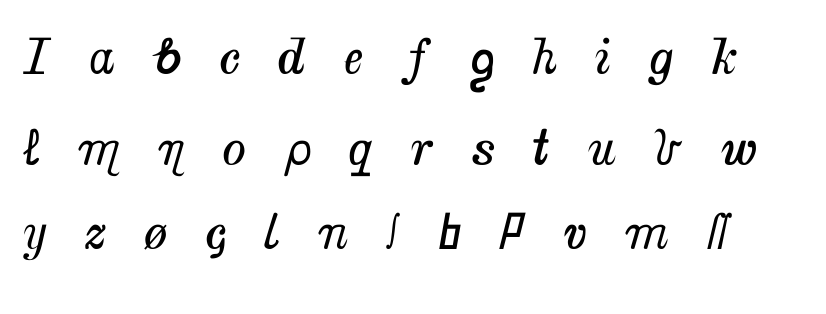
\includegraphics[width=1.00\hsize]{img/02_Parkosz_codepoints_bare}
  \caption{Repertuar fontu \texttt{Parkosz} (autor Maciej Strzelczyk)}
  \label{fig:Strzelczyk}
\end{figure}

\begin{figure}[th]
  \centering
  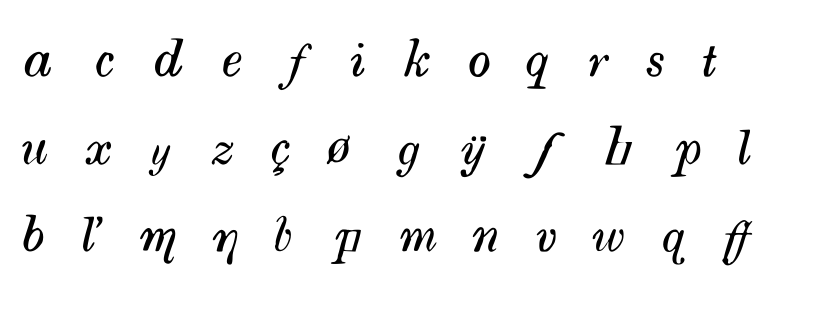
\includegraphics[width=1.00\hsize]{img/03_Parkosz_codepoints1907_bare}
  \caption{Repertuar fontu \texttt{Parkosz1907} (autor Janusz
    S. Bień)}
  \label{fig:parkosz1907}
\end{figure}

\begin{figure}[th]
  \centering
  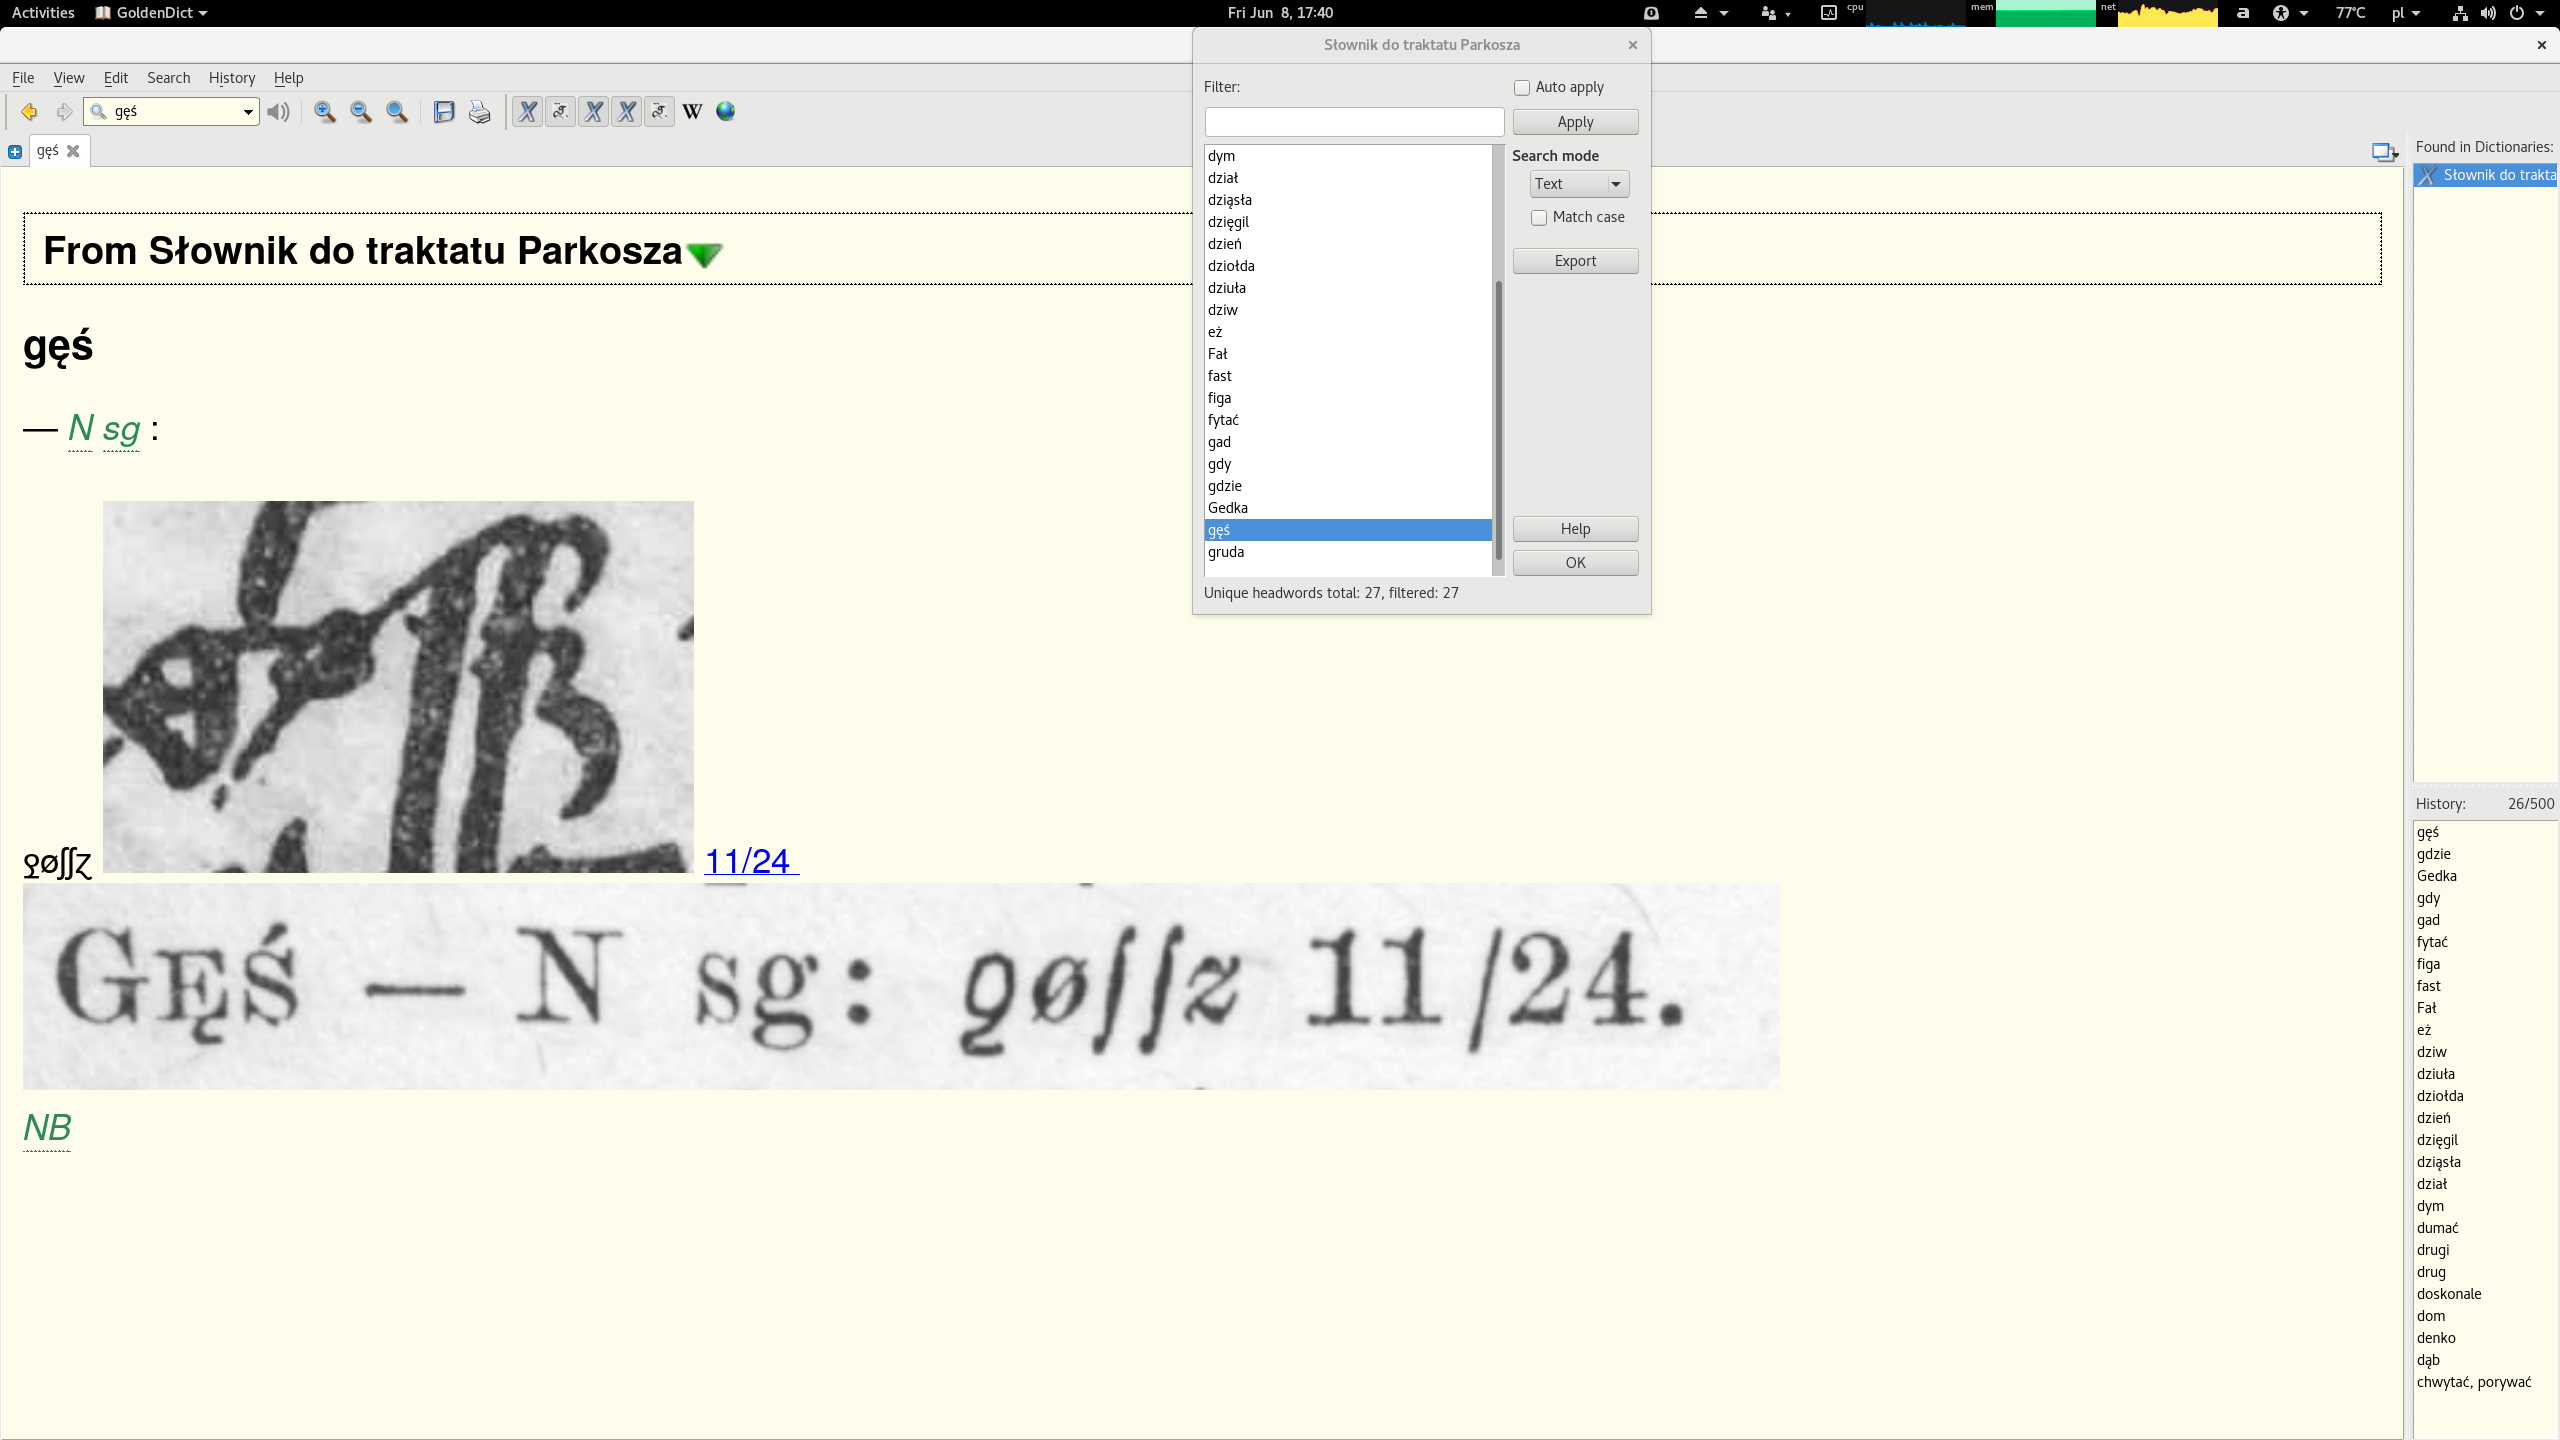
\includegraphics[width=1.00\hsize]{img/04_GoldenDict}
  \caption{Indeks wyrazów jako słownik elektroniczny (program GoldenDict)}
  \label{fig:GoldenDict}
\end{figure}

\begin{figure}
  \centering
  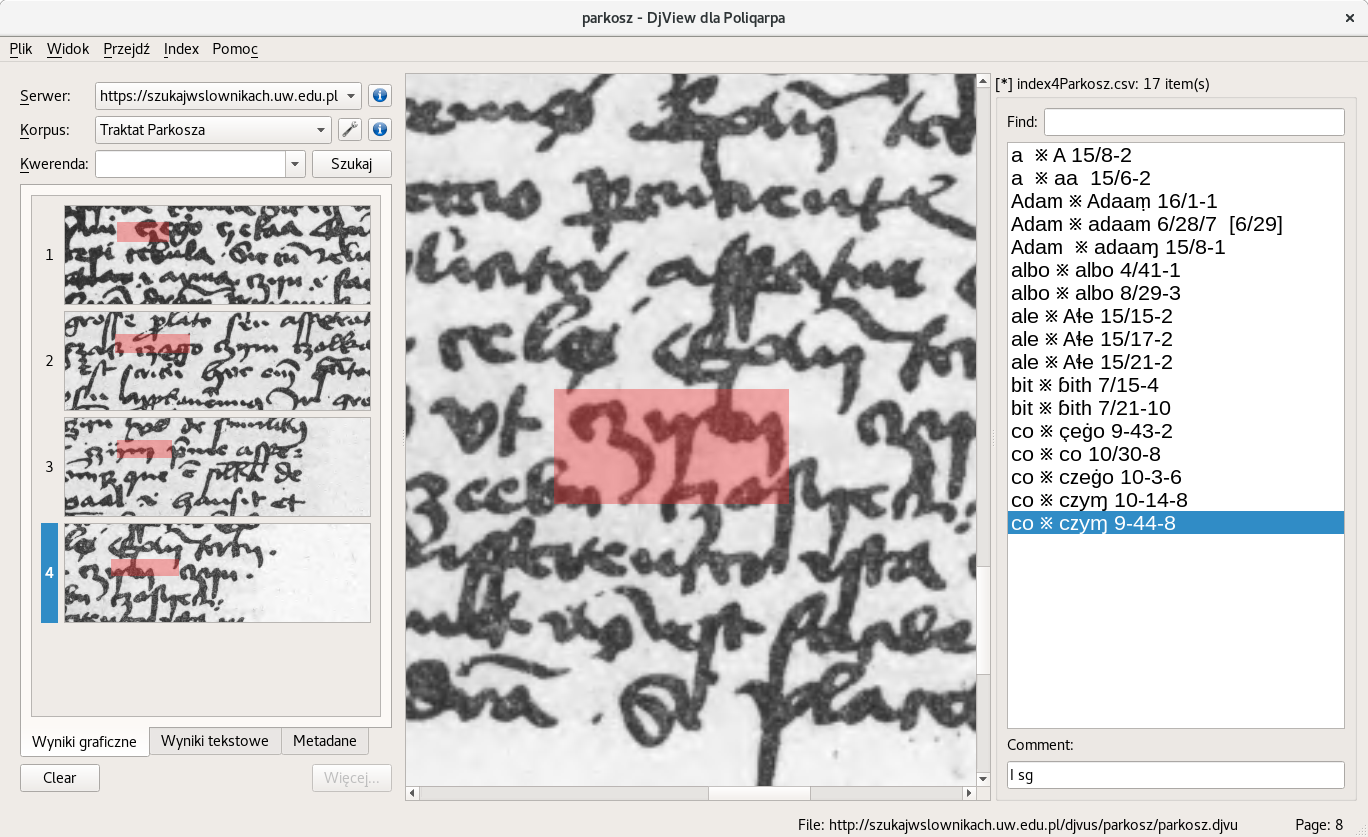
\includegraphics[width=1.00\hsize]{img/05_czymParkosz}
  \caption{Indeks wyrazów --- program \textsf{djview4poliqarp}}
  \label{fig:indeks}
\end{figure}

Piętnastowieczny rękopiśmienny łaciński traktat Parkosza jest
pierwszym tekstem poświęconym pisowni polskiej, z tego powodu znanym i
często cytowanym ---także dlatego, ze proponował wprowadzenie nowych
specyficznych liter. Na potrzeby krytycznej edycji opublikowanej w
1907 r. najwyraźniej odlano specjalne czcionki. Na potrzeby krytycznej
edycji opublikowanej w 1985 r. nietypowe znaki zostały narysowane
przez grafika, a następnie prawie cała redakcja brała udział
we wklejaniu około dwóch tysięcy wycinków we właściwe miejsca
tekstu. W czasach edycji elektronicznych sytuacja wygląda lepiej tylko
teoretycznie, jak opisałem to szczegółowo w artykule
[\cite{bien_parkoszPSP}].

W 2013 r. próbę stworzenia fontu dla traktatu Parkosza podjął mój
student Maciej Strzelczyk
\footnote{\url{https://bitbucket.org/jsbien/parkosz-font-old}.}
% \break
(por. il. \ref{fig:Strzelczyk}); wzorował się on na kształtach liter z
edycji z 1985 r.  Później samodzielnie spróbowałem stworzyć font
wzorowany na czcionkach z edycji z 1907
r.\footnote{\url{https://bitbucket.org/jsbien/parkosz-font/}.}
--- por. il. \vref{fig:parkosz1907}; obecnie uważam to za błąd ---
ponieważ chodzi o rękopis, czcionki powinny być kursywne, jak w edycji
z 1985 r. Niestety żaden z tych tworzonych nieprofesjonalnie fontów
nie może być zalecany do użytku ze względu na niesatysfakcjonującą
jakość. Nowym elementem w sprawie jest udostępnienie w Internecie
przez Bibliotekę Jagiellońską dobrej jakości skanu oryginału --- patrz np.
\url{https://jsbien.github.io/Parkosz4IIIF/}. Istnieje też
niedokończony elektroniczny indeks wystąpień poszczególnych polskich
słów w rękopisie, dostępny w dwóch formach --- patrz
il.~\ref{fig:GoldenDict} i il.~\ref{fig:indeks}
(\url{https://bitbucket.org/jsbien/parkosz-traktat/}). Można więc
przeanalizować kształt liter i przemyśleć, jak oddać je w foncie.


Ze względu na brak odpowiedniego fontu w eksperymentalnym wydaniu
elektronicznym zastosowałem transliterację szczegółowo opisaną we
wspomnianym artykule [\cite{bien_parkoszPSP}]. W stosunku do
poprzednich edycji wprowadziłem pewną innowację: litery, które mają
standardowy kształt, ale u Parkosza wymawiają się inaczej, są również
transkrybowane --- na przykład zamiast zwykłego \textit{m} (które u
Parkosza oznacza zawsze spółgłoskę miękką) stosuję \textit{ṃ}
(\uname{LATIN SMALL LETTER M WITH DOT BELOW}).

Obecnie zastosowałbym inna konwencję, mniej lub bardziej inspirowaną
czasem dość ekscentrycznymi propozycjami, które na liście dyskusyjnej
standardu Unicode
(\url{http://www.unicode.org/mailman/listinfo/unicode}) zgłasza
William Overington
(np. \url{https://forum.high-logic.com/viewtopic.php?f=10&t=7831}). Mianowicie
każdy znak z transkrybowanego alfabetu Parkosza --- niezależnie od
tego, czy jest stosowany współcześnie czy nie --- łączyłbym ze znakiem
\uname{COMBINING TRIPLE UNDERDOT},
np. {\fontspec{STIXGeneral-Italic}\textit{m⃨}}; powód, dlaczego nie
zrobiłem tego wcześniej jest prosty --- dopiero niedawno zauważyłem,
że taki znak istnieje. Dałoby to wyrazistą transkrypcję alfabetu
Parkosza, a po stworzeniu odpowiedniego fontu można by wykorzystać
mechanizm ligatur do zastępowania tych sekwencji przez właściwe glify.

\section{Analiza przypadku --- Nowy Karakter Polski}
\label{sec:anal-przyp-nowy}

Opublikowany w 1594 r. przez Jana Januszowskiego traktat \textit{Nowy
  Karakter Polski} porównuje 3 propozycje pisowni polskiej: własną,
Jana Kochanowskiego i Łukasza Górnickiego, używa przy tym
zaprojektowanego przez siebie fontu. Jego skany są obecnie dostępne we
wielu bibliotekach cyfrowych, najwygodniej udostępnia je moim zdaniem
Dolnośląska Biblioteka Cyfrowa
(\url{https://www.dbc.wroc.pl/publication/4239}).

\begin{figure}[h]
  \centering
  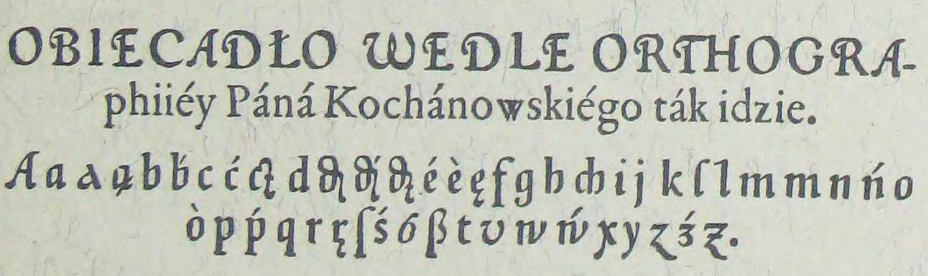
\includegraphics[width=1.00\hsize]{img/06_iNKPo54}
  \caption{Pisownia Jana Kochanowskiego (s. G3)}
  \label{fig:NKP054}
\end{figure}

\begin{figure}[h]
  \centering
  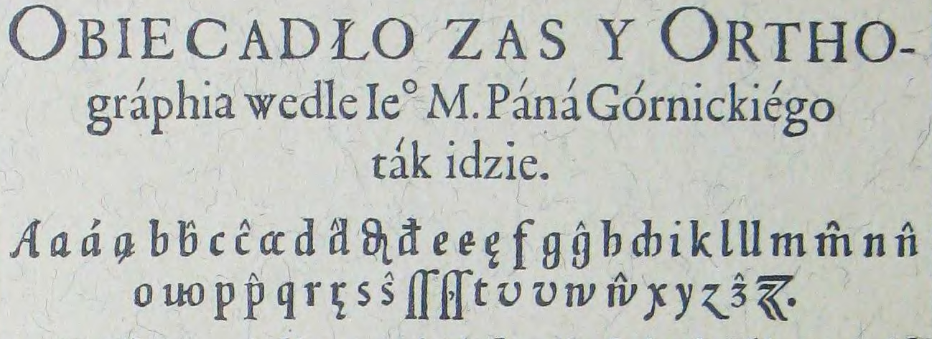
\includegraphics[width=1.00\hsize]{img/07_iNKPo55}
  \caption{Pisownia Łukasza Górnickiego (s. G3v)}
  \label{fig:NKP055}
\end{figure}


\begin{figure}[h]
  \centering
  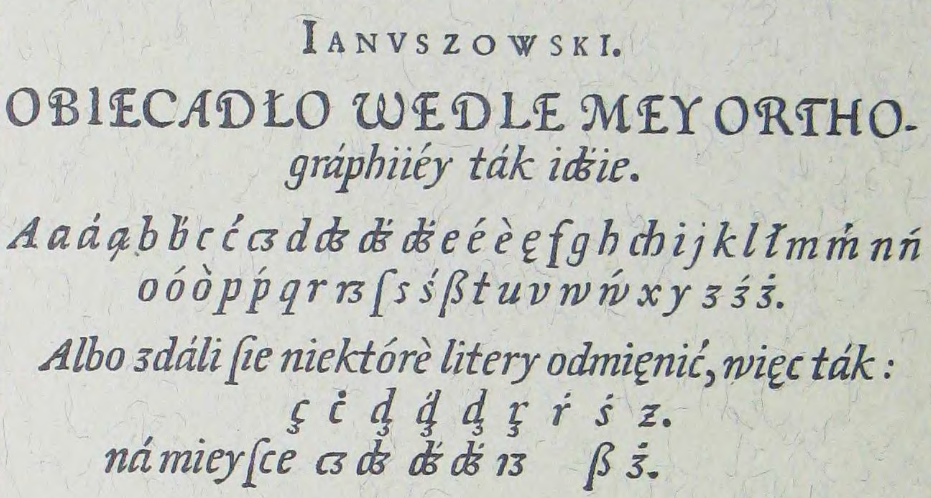
\includegraphics[width=1.00\hsize]{img/08_iNKPo63}
  \caption{Pisownia Jana Januszowskiego (s. H3v)}
  \label{fig:NKP063}
\end{figure}

Dygitalizacja tego traktatu
stanowi duże wyzwania ze względu na dużą liczbę znaków, które nie są
współcześnie używane. Stwarza to szereg problemów, z których
najbardziej rzuca się w oczy potrzeba odpowiedniego fontu do
prezentacji tych znaków.

Pierwsza znana dygitalizacja fontu Januszowskiego to font
\textit{FAKarakter} Artura Frankowskiego stworzony chyba w 1995 r. Na
pytanie o dostępność fontu otrzymałem w 2010 r. odpowiedź
\textit{Obecnie dostępna jest jedna odmiana kroju FA Karakter.  Jeden
  font (odmiana) kosztuje 90 zł netto. Powyższe cena dotyczy licencji
  na jedno stanowisko komputerowe dla jednego nabywcy.} Na pytanie,
jaki jest repertuar znaków i jaki format, nie otrzymałem nigdy
odpowiedzi.

% To: fontarte <studio@fontarte.com>
% Subject: Re: FA Karakter
% From: jsbien@mimuw.edu.pl (Janusz S. Bień)
% Gcc: nnfolder+archive:sent.2019-06
% Reply-to: jsbien@mimuw.edu.pl
% Bcc: jsbien@mimuw.edu.pl
% --text follows this line--
% On Tue, Apr 20 2010 at 12:42 +02, fontarte wrote:
% > Dzień dobry,
% > Przepraszam za opowiedz po tak długim okresie, ale byłem w podróży służbowej i dopiero dziś mogłem odpisać.
% >
% > Obecnie dostępna jest jedna odmiana kroju FA Karakter.
% > Jeden font (odmiana) kosztuje 90 zł netto. Powyższe cena dotyczy licencji na jedno stanowisko komputerowe dla jednego nabywcy.
% >
% > Oto ceny jednej odmiany (fontu) w zależności od liczby stanowisk:
% >
% > il. stanowisk / cena netto 
% > --------------------------------
% > 1 / 90 zł
% > 2-5 / 150 zł
% > 6-10 / 280 zł
% > 11- 25 / 465 zł
% > --------------------------------
% >
% > W przypadku decyzji o zakupie proszę o maila (dla kogo faktura) i przelew na konto:
% > mBank 87 1140 2004 0000 3202 39779110
% > Fontarte s.c.
% > ul. Opoczyńska 1/3
% > 02-522 Warszawa
% > (tytuł przelewu: FA Karakter/nazwa kupujacego) 
% >
% > Po otrzymaniu wpłaty, przesyłamy mailem fonty oraz fakturę VAT.
% >
% > Pozdrawiam,
% >
% > Artur Frankowski
% >
% > : : : : : : : : : : : : : : : : : : : : : : : : : 
% > FONTARTE | design & fonts |
% > + 48 22 646 98 53
% > mobile: 693 70 00 11
% > http://www.fontarte.com
% >
% > On Apr 11, 2010, at 6:56 AM, Janusz S. Bień wrote:
% >
% >  Witam!
% >
% >  Interesuję się dygitalizacją dawnych tekstów polskich, por. np.
% >
% >             http://bc.klf.uw.edu.pl/71/
% >
% >  W związku z tym chciałbym zapytać, czy font
% >
% >      http://free.art.pl/magdart/karakter.htm
% >
% >  jest jakoś dostępny?
% >
% >  Z poważaniem
% >
% >  JSB
% >
% >  -- 
% >                       ,   
% >  dr hab. Janusz S. Bien, prof. UW -  Uniwersytet Warszawski (Katedra Lingwistyki Formalnej)
% >  Prof. Janusz S. Bien - Warsaw University (Department of Formal Linguistics)
% >  jsbien@uw.edu.pl, jsbien@mimuw.edu.pl, http://fleksem.klf.uw.edu.pl/~jsbien/
% >

% On Wed, Apr 21 2010 at 13:41 +02, Janusz S. Bień wrote:
% > On Tue, 20 Apr 2010  fontarte <studio@fontarte.com> wrote:
% >
% > [...]
% >
% >> Obecnie dostępna jest jedna odmiana kroju FA Karakter.
% >> Jeden font (odmiana) kosztuje 90 zł netto. Powyższe cena dotyczy  
% >> licencji na jedno stanowisko komputerowe dla jednego nabywcy.
% >
% > A jaki jest format fontu i repertuar znaków?
% >
% > [...]
% >
% >> Po otrzymaniu wpłaty, przesyłamy mailem fonty oraz fakturę VAT.
% >
% > Gdybym się zdecydował kupić, to 1 licencję dla Katedry, ale my płacimy
% > przelewem w ciągu 2 tygodni od otrzymania faktury.
% >
% > Z poważaniem
% >
% > JSB

% On Mon, Jul 16 2018 at  7:03 +02, Janusz S. Bień wrote:
% > Szanowny Panie!
% >
% > Na poniższy list nie otrzymałem niestety odpowiedzi:
% >
% > On Wed, Apr 21 2010 at 13:41 +0200, jsbien@mimuw.edu.pl writes:
% >> On Tue, 20 Apr 2010  fontarte <studio@fontarte.com> wrote:
% >>
% >> [...]
% >>
% >>> Obecnie dostępna jest jedna odmiana kroju FA Karakter.
% >>> Jeden font (odmiana) kosztuje 90 zł netto. Powyższe cena dotyczy  
% >>> licencji na jedno stanowisko komputerowe dla jednego nabywcy.
% >>
% >> A jaki jest format fontu i repertuar znaków?
% >>
% >> [...]
% >>
% >>> Po otrzymaniu wpłaty, przesyłamy mailem fonty oraz fakturę VAT.
% >>
% >> Gdybym się zdecydował kupić, to 1 licencję dla Katedry, ale my płacimy
% >> przelewem w ciągu 2 tygodni od otrzymania faktury.
% >>
% >> Z poważaniem
% >>
% >> JSB
% >
% > Czy nadal oferuje Pan font na warunkach opisanych w poniższym mejlu?
% >
% > On Tue, Apr 20 2010 at 12:42 +0200, studio@fontarte.com writes:
% >> Dzień dobry,
% >> Przepraszam za opowiedz po tak długim okresie, ale byłem w podróży służbowej i dopiero dziś mogłem odpisać.
% >>
% >> Obecnie dostępna jest jedna odmiana kroju FA Karakter.
% >> Jeden font (odmiana) kosztuje 90 zł netto. Powyższe cena dotyczy licencji na jedno stanowisko komputerowe dla jednego nabywcy.
% >>
% >> Oto ceny jednej odmiany (fontu) w zależności od liczby stanowisk:
% >>
% >> il. stanowisk / cena netto 
% >> --------------------------------
% >> 1 / 90 zł
% >> 2-5 / 150 zł
% >> 6-10 / 280 zł
% >> 11- 25 / 465 zł
% >> --------------------------------
% >>
% >> W przypadku decyzji o zakupie proszę o maila (dla kogo faktura) i przelew na konto:
% >> mBank 87 1140 2004 0000 3202 39779110
% >> Fontarte s.c.
% >> ul. Opoczyńska 1/3
% >> 02-522 Warszawa
% >> (tytuł przelewu: FA Karakter/nazwa kupujacego) 
% >>
% >> Po otrzymaniu wpłaty, przesyłamy mailem fonty oraz fakturę VAT.
% >>
% >> Pozdrawiam,
% >>
% >> Artur Frankowski
% >>
% >> : : : : : : : : : : : : : : : : : : : : : : : : : 
% >> FONTARTE | design & fonts |
% >> + 48 22 646 98 53
% >> mobile: 693 70 00 11
% >> http://www.fontarte.com
% >>
% >> On Apr 11, 2010, at 6:56 AM, Janusz S. Bień wrote:
% >>
% >>  Witam!
% >>
% >>  Interesuję się dygitalizacją dawnych tekstów polskich, por. np.
% >>
% >>  http://bc.klf.uw.edu.pl/71/
% >>
% >>  W związku z tym chciałbym zapytać, czy font
% >>
% >>  http://free.art.pl/magdart/karakter.htm
% >>
% >>  jest jakoś dostępny?
% >>
% >>  Z poważaniem
% >>
% >>  JSB
% >>
% >>  -- 
% >>  , 
% >>  dr hab. Janusz S. Bien, prof. UW - Uniwersytet Warszawski (Katedra Lingwistyki Formalnej)
% >>  Prof. Janusz S. Bien - Warsaw University (Department of Formal Linguistics)
% >>  jsbien@uw.edu.pl, jsbien@mimuw.edu.pl, http://fleksem.klf.uw.edu.pl/~jsbien/
% >
% > Czy w ogóle ktokolwiek go kupił?
% >
% > Tym razem ja nie zamierzam jednak go kupować, a jedynie uaktualnić
% > informację w Wikipedii, która - choć prawdziwa - jest moim zdaniem
% > myląca:
% >
% > https://pl.wikipedia.org/wiki/Nowy_karakter_polski
% >
% > W razie braku odpowiedzi umieszczę w Wikipedii informację, że font nie
% > jest obecnie udostępniany w żadnej formie.
% >
% > Z poważaniem
% >
% > JSB

Wiadomo też, że font zdigitalizował Paweł Osial
[\cite[39]{anna_wielunska_digitalizacja_2018}] na potrzeby swojej
pracy dyplomowej; repertuar znaków nie jest mi znany.


Względnie dobrze udokumentowana jest rodzina fontów, które stworzyła
Anna Wieluńska. Proces ich tworzenia został opisany artykule
[\cite{anna_wielunska_digitalizacja_2018}] będący omówieniem jej pracy
magisterskiej, opublikowanej w wersji rozszerzonej jako
[\cite{wielunska_anna_lazarus:_2018}].  Tej rodzinie fontów, nazwanej
Lazarus, poświęcona jest witryna \url{https://www.lazarus.wtf}.


W pracy [\cite[52]{wielunska_anna_lazarus:_2018}] znajdujemy stwierdzenie
  \textit{Projekt i rozbudowa historycznych odmian odlanych przez
  Januszowskiego (\textit{italic}, \textit{upright italic}) zostały
  dofinansowane w ramach stypendium Ministra Kultury i Dziedzictwa
  Narodowego i zostaną udostępnione na otwartej licencji.}
Aktualnie są one jednak dostępne --- o ile mi wiadomo --- tylko na
stronie \url{https://capitalics.wtf/pl/font/lazarus} na zasadach
\textit{Licencji Darmowej} (\url{https://capitalics.wtf/pl/licence}),
która licencją otwartą nie jest. Pozostałe dwa fonty są dostępne w
cenie 123 zł każdy (cały komplet kosztuje 153,75 zł).

Repertuar znaków został uwspółcześniony. Na stronach 58-59, 66-67 i
74-75 znajdują się porównania stron oryginału z tekstem złożonym
fontami z rodziny Lazarus. Najbardziej rzuca się w oczy brak znaków
wymaganych przez pisownię Kochanowskiego. Inne różnice to pewnie też
świadome decyzje projektowe: współczesny kształt liter \textit{k} i
\textit{r}, nosówek \textit{ą} i \textit{ę} (w oryginale przekreślenia
zamiast ogonków), współczesny dywiz używany do dzielenia również słów
w gotyku (zamiast \textsc{double oblique hyphen}), współczesny ukośnik
zamiast \label{virgula}\textsc{short virgula} (M+F1F1), odróżnianie
\textit{u} i \textit{v}. Niektóre różnice to po prostu przeoczenia
autorki --- tak chyba trzeba zaklasyfikować np. brak diakrytu nad
\textit{e} w trzecim wierszu od góry na s. 58.

% „Nowy karakter polski” z 1594 roku, autorstwa Jana Januszowskiego,
% Jana Kochanowskiego i Łukasza Górnickiego był jedną z pierwszych w
% historii prób zunifikowania systemu zapisu języka polskiego. Wszystkie
% teksty w nim zawarte, zostały złożone nowym, autorskim systemem - na
% potrzeby rozważań nad ortografią, Januszowski opracował i odlał dwie
% nowe czcionki - karakter prosty i pochyły.

% Lazarus to rodzina 4 krojów, zdigitalizowanych na podstawie czcionek
% „Nowego Karakteru”. Praca nad projektem trwała ponad dwa lata i
% zakładała długie i wnikliwe badania nad oryginałem, opracowanie
% autorskiej metody digitalizacji oraz znaczną rozbudowę orygianlnych
% zestawów znaków. Cały proces został opisany w teoretycznej pracy
% magisterskiej pod kierunkiem prof. Doroty Folgi-Januszewskiej (pdf na
% stronie www.lazarus.wtf), natomiast kroje powstały jako część
% praktycznej pracy dyplomowej, pod czujnym okiem Michała Jarocińskiego
% w Typowej Pracowni. Praca dyplomowa której częścią był Lazarus
% otrzymała wyróżnienie rektorskie oraz była pokazywana na wystawie
% najlepszych dyplomów warszawskiej Akademii Sztuk Pięknych - Coming Out
% 2017.

% Finalny zestaw krojów składa się z dwóch historyzujących odmian,
% powstałych na bazie projektu Januszowskiego - Italic i Upright Italic
% (karaktery prosty i pochyły), z antykwy (regular), która stanowi
% interpretację atykwy użytej przez Januszowskiego do składu łacińskich
% tekstów oraz z fraktury, będącej luźną interpretacją czcionki Mytel
% Polski, która również została wykorzystana przy składzie „Nowego
% Karakteru”. Wszystkie cztery odmiany posiadają pełen zestaw znaków dla
% łaciny (WE, CE, SEE), Italic ma bogaty zestaw ozdobnych setów
% stylistycznych, zaś Regular detaliczne ornamenty i zestaw
% rączek. Rodzina ze względu na swój historyczny charakter świetnie
% sprawdzi się w klasycznych sytuacjach, ale nie oprze się również
% eksperymentom!

% Projekt odmian Italic i Upright Italic został dofinansowany w ramach stypendium Ministra Kultury i Dziedzictwa Narodowego.

% https://lazarus.wtf/

% Kliknięcie przeniesie Cię na stronę Capitalics.wtf z której można
% pobrać za darmo 2 historyczne odmiany (Italic i Upright Italic) oraz
% kupić 2 odmiay dopełniające.

% Poza historycznymi odmianami zaprojektowanymi i odlanymi przez
% Januszowskiego, Lazarus ma jeszcze dwie odmiany, bazujące na
% wykorzystywanych w oryginalnej broszurze z 1594 roku – Regular i
% Fraktur. Jednym z głównych celów projektu było dopasowanie do siebie
% rysunku wszystkich odmian tak, aby mogły działać razem jako
% uzupełniająca się całość. Finalne style przechodzą od najbardziej
% miękkiego (Regular) do ostrego (Fraktur). Odmiana Upright italic
% stanowi przejście pomiędzy Italikiem a Frakturą. Fraktura luźno bazuje
% na czcionce, którą można odnaleźć we wzorniku czcionek Akademii
% Zamojskiej, oznaczonej Mytel Polski, zachowując detale wypracowane
% przy okazji reszty odmian.

% https://lazarus.wtf/

O wspomnianej we wstępie dygitalizacji fontów \textit{Nowego karakteru
  polskiego} uwzględniającej m.in. znaki pisowni proponowanej przez
Jana Kochanowskiego wiadomo niestety bardzo mało: została wykonana pod
kierunkiem Bogdana Hojdisa, jej autorami są Monika Marek-Łucka i
Damian Langosz; nie wiadomo, czy font jest dostępny publicznie, a
jeśli tak, to na jakiej licencji. Niewielka próbka dostępna jest w
artykule [\cite[9]{hojdis_problemy_2016}],% (Rys. 4),
nieco większa na
slajdzie cytowanym w sprawozdaniu z konferencji \textit{Tekstologia i
  typografia w przestrzeni cyfrowej} (Toruń 2015), gdzie artykuł ten
był referowany --- patrz [\cite[73]{pest15:_t_t}]. Sprawozdanie cytuje
też bardzo trafne stwierdzenie referenta [Bodana Hojdisa]
\textit{najtrudniejszym problemem do rozwiązania pozostaje jednak samo
  kodowanie staropolskich znaków, dla których nie przewidziano miejsca
  w międzynarodowym standardzie Unicode} [\cite[72]{pest15:_t_t}].


Instytut Badań Literackich PAN, który jest odpowiedzialny za wydanie
sejmowe dzieł wszystkich Jana Kochanowskiego, od 1948 r. prowadzi
również prace nad \textit{Słownikiem polszczyzny XVI wieku}, ukazało
się dotąd 37 tomów (łącznie około 20 tysięcy stron)\footnote{W
  2020~r. ukazały się 3 zeszyty tomu 38 [Uwaga dodana we wrześniu 2020
  r.]}. \textit{Nowy Karakter Polski} jest cytowany w treści słownika,
a nietypowe litery są oddawane w sposób zależny od zastosowanej
technologi składu --- jak widać, wierne cytowanie oryginału jest
istotne przynajmniej dla niektórych polonistów.

% /mnt/MyBookT2/jsbien/structure.txt

% \footnote{Pomimo stworzenia w Instytucie Centrum Humanistyki
%   Cyfrowej obieg informacji w tej instytucji nie wygląda najlepiej ---
%   redakcja słownika dowiedziała sie o istnieniu ,,fontu Hojdisa''
%   dopiero ode mnie w 2019 r.}.


\begin{figure}[h]
  \centering
  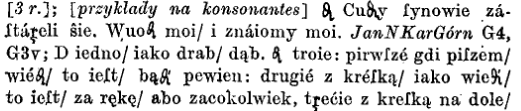
\includegraphics[width=1.00\hsize]{img/09_Czytelnia_006_06_001s315b}
  \caption{SpXVIw t. VI (1972) s. 303 --- skład monotypowy}
  \label{fig:SpXVIw6-303}
\end{figure}

\begin{figure}[h]
  \centering
  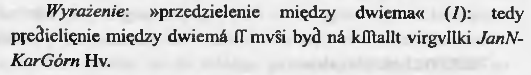
\includegraphics[width=1.00\hsize]{img/10_Czytelnia_011_11s314virgulki}
  \caption{SpXVIw t. XXXI (2003) s. 221 --- skład komputerowy (Kombi)}
 % \caption{Czytelnia_011_11s314virgulki}
  \label{fig:SpXVIw31-221}
\end{figure}

\begin{figure}[h]
  \centering
  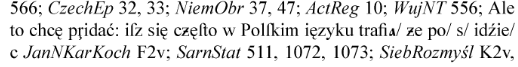
\includegraphics[width=1.00\hsize]{img/11_spxviw-33s174}
  \caption{SpXVIw t. XXXIII (2009) s. 172 --- skład komputerowy (Kombi)}
  \label{fig:SpXVw33-174}
\end{figure}

\begin{figure}[h]
  \centering
  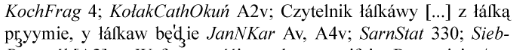
\includegraphics[width=1.00\hsize]{img/12_spxviw-33s273.png}
  \caption{SpXVIw t. XXXIII (2009) s. 261 --- skład komputerowy (Kombi)}
  \label{fig:SpXVIw33-261}
\end{figure}


% ,,biblioteka'' mój pomysł cytowany przez Saloniego

% Wynik realizacji projektu badawczego finansowanego ze środków NPRH
% pt. "Korpus polszczyzny XVI wieku. Etap I: digitalizacja źródeł oraz
% stworzenie narzędzi informatycznych i udostępnienie materiałów
% testowych korpusu" realizowanego w latach 2012-2017 w Pracowni
% Słownika Polszczyzny XVI wiek IBL PAN ; 53 s.


Redakcja słownika w ramach grantu NPRH nr 0138/FNiTP/H11/80/2011
\textit{Korpus polszczyzny XVI wieku. Etap I: digitalizacja źródeł
  oraz stworzenie narzędzi informatycznych i udostępnienie materiałów
  testowych korpusu} realizowanego w latach 2012-2017 opublikowała w
wersji elektronicznej kilka pozycji serii \textit{Biblioteka źródeł
  Słownika polszczyzny XVI wieku. Repozytorium cyfrowe tekstów
  szesnastowiecznych (w jednolitej transliteracji zgodnej z Zasadami
  wydawania tekstów staropolskich (projekt), Wrocław
  1955\footnote{Stwierdzenie to nie jest w pełni prawdziwe, ale
    najwyraźniej nikomu to nie przeszkadza.})} pod redakcją Patrycji
Potoniec i Krzysztofa Opalińskiego (ISBN 978-83-65832-90-0), w
szczególności kilka pozycji podserii \textit{Słowniki i gramatyki} w
opracowaniu Anny Nath-Dokurno, Patrycji Potoniec i Piotra Małka.
%(całość) ISBN 978-83-65832-09-2
W podserii tej ukazał się również \textit{Nowy karakter Polski} (ISBN
978-83-65832-09-2) dostępny w wersji PDF w Repozytorium Cyfrowym
Instytutów Naukowych (\url{http://rcin.org.pl/publication/82568}, a w
formie HTML pod adresem
\url{http://spxvi.edu.pl/korpus/teksty/JanNKar/}
%   dopiero ode mnie w 2019 r.}.
Teksty zakodowane są zgodnie ze standardem Unicode z wykorzystaniem
znaków prywatnych z rekomendacji MUFI. Wykorzystywany jest font
Polemonas MUFI, który można pobrać--- w kilku odmianach --- z witryny
MUFI (\url{https://folk.uib.no/hnooh/mufi/fonts/}; nie należy go mylić
z fontem Polemonas
(\url{https://klevas.mif.vu.lt/~vladas/Palemonas.htm}), przeznaczonym
specjalnie dla języka litewskiego. Problem niedostępnych znaków
rozwiązano stosując transkrypcję, przy czym transkrybowane fragmenty
są wyróżnione kolorem --- patrz ilustracje \vref{fig:NKP054html},
\vref{fig:NKP055html}, \vref{fig:NKP063html}, \vref{fig:NKP054pdf},
\vref{fig:NKP055pdf}, \vref{fig:NKP063pdf}.


\begin{figure}[h]
  \centering
  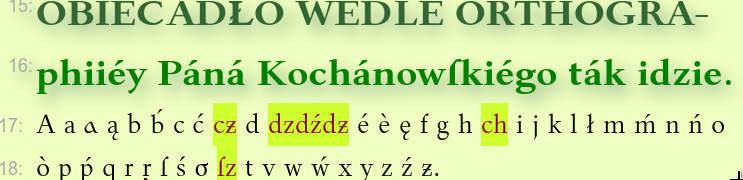
\includegraphics[width=1.00\hsize]{img/13_KochanowskiHTML}
  \caption{Transkrypcja --- HTML: pisownia Jana Kochanowskiego (s. G3)}
  \label{fig:NKP054html}
\end{figure}

\begin{figure}[h]
  \centering
  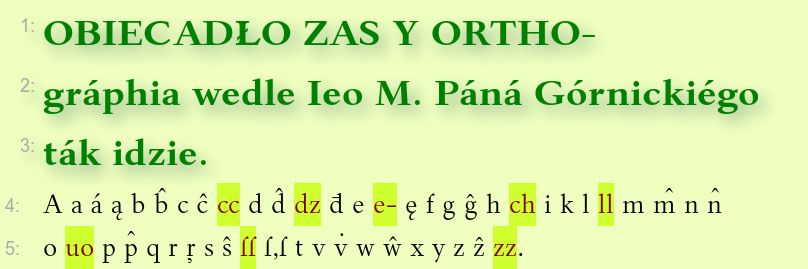
\includegraphics[width=1.00\hsize]{img/14_GornickiHTML}
  \caption{Transkrypcja --- HTML: pisownia Łukasza Górnickiego (s. G3v)}
  \label{fig:NKP055html}
\end{figure}


\begin{figure}[h]
  \centering
  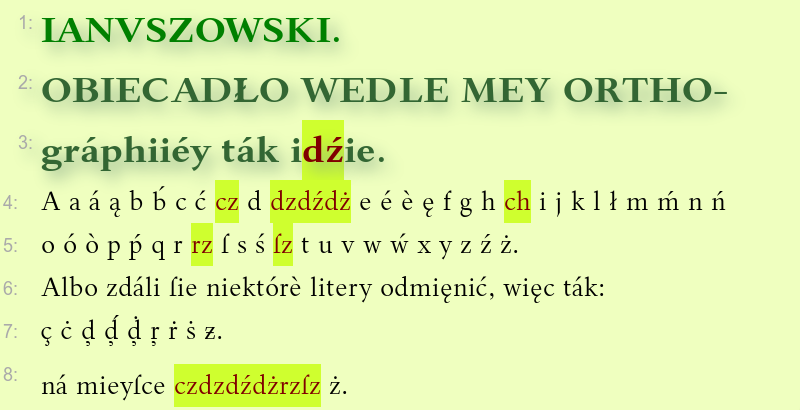
\includegraphics[width=1.00\hsize]{img/15_JanuszowskiHTML}
  \caption{Transkrypcja --- HTML: pisownia Jana Januszowskiego (s. H3v)}
  \label{fig:NKP063html}
\end{figure}

\begin{figure}[h]
  \centering
  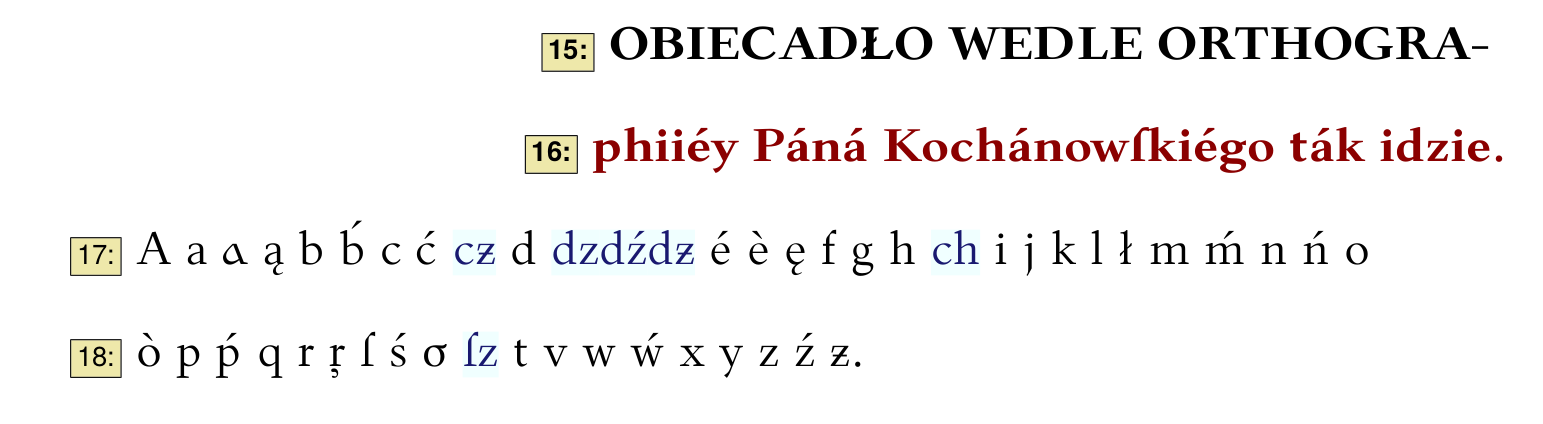
\includegraphics[width=1.00\hsize]{img/16_KochanowskiPDF}
  \caption{Transkrypcja --- PDF: pisownia Jana Kochanowskiego (s. G3)}
  \label{fig:NKP054pdf}
\end{figure}

\begin{figure}[h]
  \centering
  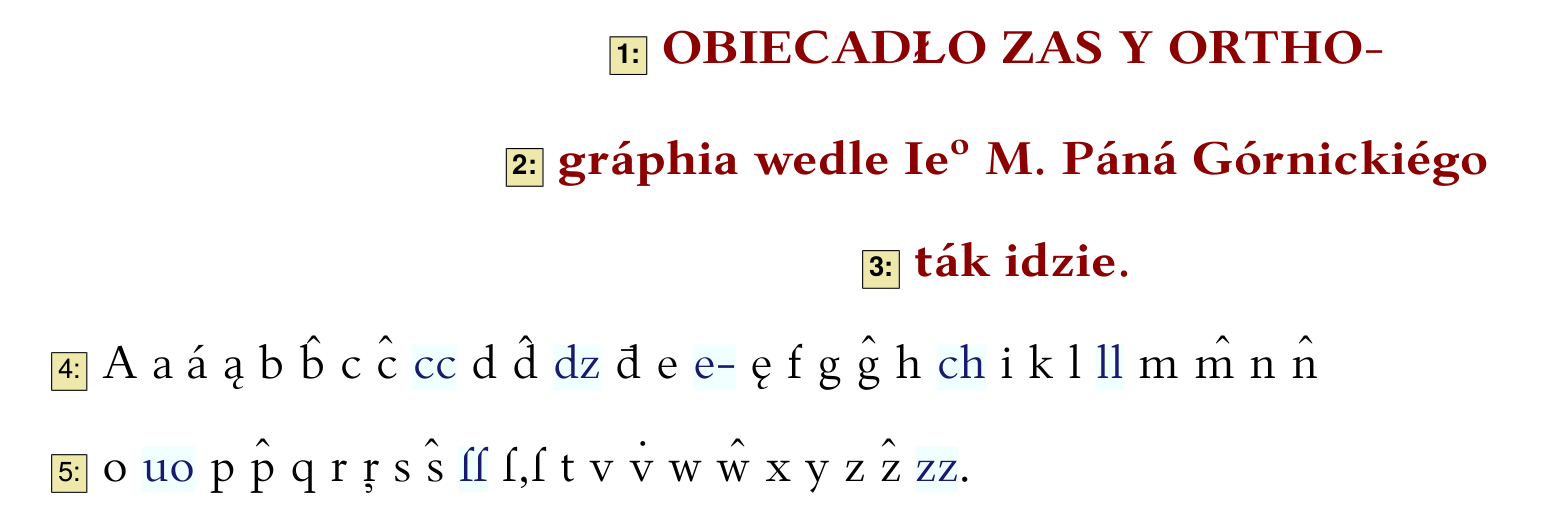
\includegraphics[width=1.00\hsize]{img/17_GornickiPDF}
  \caption{Transkrypcja --- PDF: pisownia Łukasza Górnickiego (s. G3v)}
  \label{fig:NKP055pdf}
\end{figure}


\begin{figure}[h]
  \centering
  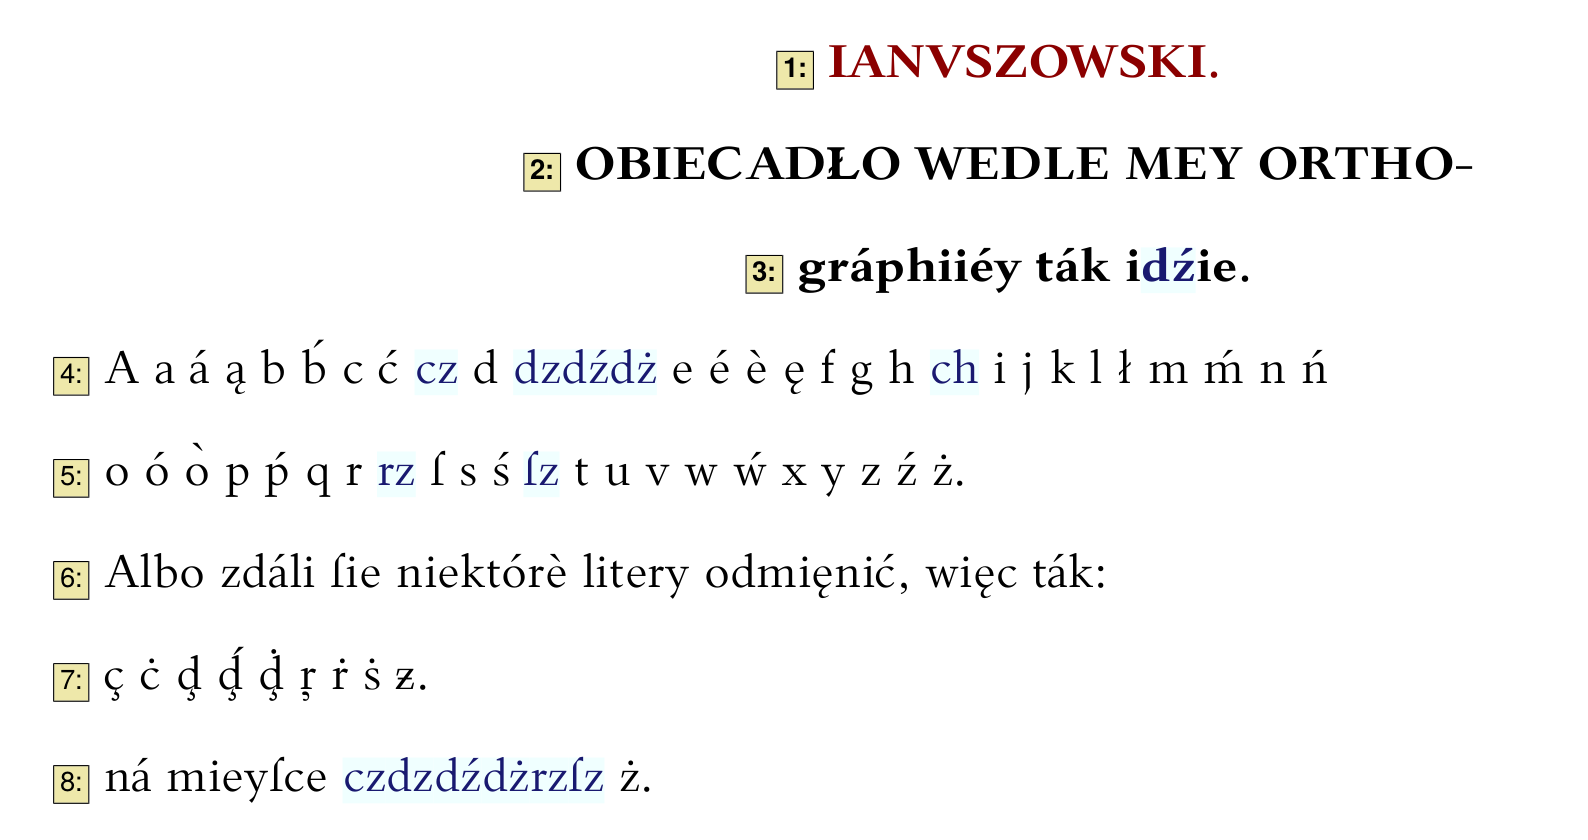
\includegraphics[width=1.00\hsize]{img/18_JanuszowskiPDF}
  \caption{Transkrypcja --- PDF: pisownia Jana Januszowskiego (s. H3v)}
  \label{fig:NKP063pdf}
\end{figure}

% https://folk.uib.no/hnooh/mufi/fonts/
% Regular | Italic | Bold | Bold italic

% ,,biblioteka'' mój pomysł cytowany przez Saloniego

% Biblioteka źródeł Słownika polszczyzny XVI wieku
% Repozytorium cyfrowe tekstów szesnastowiecznych (w jednolitej transliteracji zgodnej z Zasadami
% wydawania tekstów staropolskich (projekt), Wrocław 1955) – red. P. Potoniec, K. Opaliński
% Słowniki i gramatyki
% oprac. Anna Nath-Dokurno, Patrycja Potoniec, Piotr Małek
% ISBN 978-83-65832-90-0 (całość)
% ISBN 978-83-65832-09-2

% https://klevas.mif.vu.lt/~vladas/Palemonas.htm

% https://klevas.mif.vu.lt/~vladas/PalemonasCodeCharts.pdf

% https://github.com/pypt/Palemonas

% A a  ą b  c ć cƶ d dzdźdƶ é è ę f g h ch i j k l ł m ḿ n ń o
% 18:
% ò p ṕ q r ŗ ſ ś σ ſz t v w ẃ x y z ź ƶ.

% A a á ą b b̂ c ĉ cc d d̂ dz d e e- ę f g ĝ h ch i k l ll m m̂ n n̂
% 5:
% o uo p p̂ q r ŗ s ŝ ſſ ſ,ſ t v v̇ w ŵ x y z ẑ zz.

%   0xE444

% IANVSZOWSKI.
% 2:
% OBIECADŁO WEDLE MEY ORTHO-
% 3:
% gráphiiéy ták idźie.
% 4:
% A a á ą b  c ć cz d dzdźdż e é è ę f g h ch i j k l ł m ḿ n ń
% 5:
% o ó ò p ṕ q r rz ſ s ś ſz t u v w ẃ x y z ź ż.
% 6:
% Albo zdáli ſie niektórè litery odmięnić, więc ták:
% 7:
% ç ċ ḑ ḑ́ ḑ̇ ŗ ṙ ṡ ƶ.
% 8:
% ná mieyſce czdzdźdżrzſz ż.

\begin{figure}[h]
  \centering
  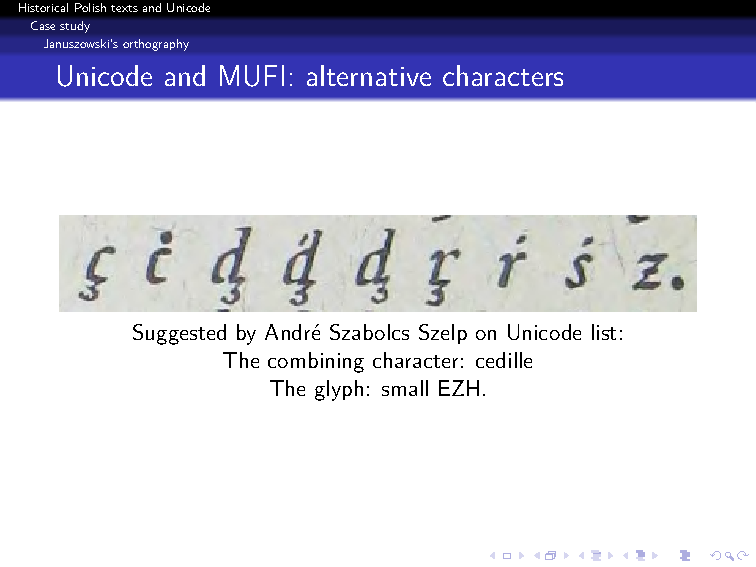
\includegraphics[width=1.00\hsize]{img/19_HPl-Unicode_slides2010-65}
  \caption{J. S. Bień \textit{Historical Polish texts and Unicode} (2011) s. 65}
  \label{fig:HPl65}
\end{figure}


% From: jsbien@mimuw.edu.pl (Janusz S. Bień)
% Subject: ,,semi-virgula''
% To: unicode@unicode.org
% Date: Mon, 30 Aug 2010 06:10:17 +0200 (8 years, 41 weeks, 5 days ago)
% Reply-to: jsbien@mimuw.edu.pl
% Attachments: [2. \"semi-virgula\" in Die Altpolnischen Orthographien --- image/png; semi-virgula.png]...
%  [3. a with stroke/semi-virgula --- image/png; a with stroke-001.png]...
%  [4. alpha with stroke/semi-virgula/caudatum --- image/png; alpha_caudatum.png]...

%  Quote/Cytat - Manuel Strehl <boldewyn@gmail.com> (Fri 17 Mar 2017
% 09:44:15 PM CET):

% > Hi,
% >
% > for my work on codepoints.net and Emojipedia I found myself repeatedly
% > in a place, where I needed some tool like hexdump to inspect the content
% > of a string. However, instead of raw bytes I am more interested in the
% > code points that the string is composed of. So I wrote this tool.

% From: jsbien@mimuw.edu.pl (Janusz S. Bień)
% Subject: preparing a PUA specification (for historical Polish text)
% To: unicode@unicode.org
% Date: Sun, 11 Apr 2010 07:32:36 +0200 (9 years, 9 weeks, 4 days ago)
% Reply-to: jsbien@mimuw.edu.pl
% Gnus-Warning: This is a duplicate of message <8739z2o8p7.fsf@mimuw.edu.pl>


% I intend to document characters used in historical Polish texts and to
% identify those of them which are absent both in Unicode and MUFI
% specifications, cf.

%       http://bc.klf.uw.edu.pl/155/

% The next stage will be to assign PUA code point to them, primarily for
% the purpose to encode the texts systematically for inclusion in the
% search engine

%      http://poliqarp.wbl.klf.uw.edu.pl/

% At this stage my question is purely technical: what is the best form
% to prepare and maintain such a specification? 

% My idea is to use at least two files, similar to UnicodeData.txt and
% NamedSequences.txt. Is this the right way to go?

% Best regards

% JSB


% From: Karl Pentzlin <karl-pentzlin@acssoft.de>
% Subject: Draft Proposal to add Variation Sequences for Latin and Cyrillic letters
% To: unicode@unicode.org
% Date: Tue, 3 Aug 2010 02:04:41 +0200 (8 years, 45 weeks, 4 days ago)
% Organization: DIN NA 043-01-35-01 GAK "Tastaturen und Eingabemittel" (keyboards and input devices), DIN NA 043-01-29-01 AK "Codierte Zeichensätze" (coded character sets)
% Reply-To: Karl Pentzlin <karl-pentzlin@acssoft.de>

% I have compiled a draft proposal:
% Proposal to add Variation Sequences for Latin and Cyrillic letters
% The draft can be downloaded at:
%  http://www.pentzlin.com/Variation-Sequences-Latin-Cyrillic2.pdf (4.3 MB).
% The final proposal is intended to be submitted for the next UTC
% starting next Monday (August 9).

% Any comments are welcome.

% - Karl Pentzlin

% From: André Szabolcs Szelp <a.sz.szelp@gmail.com>
% Subject: Re: cedille in Polish (was: preparing a PUA specification (for  historical Polish text))
% To: jsbien@mimuw.edu.pl
% Date: Sun, 18 Apr 2010 09:41:53 +0200 (9 years, 8 weeks, 4 days ago)
% Attachment: [2. text/plain]...

% Hi,

% > If Wikipedia is  correct,

% Actually, in the case of the "visigothic z" the development would be ʒ (the paleographic variant of z) > ç directly. This is -- supposedly -- attested by Old
% Spanish paleographic evidence.

% I am however quite convinced that the ç (c with cedille) in today's form has a double history (quite similar to modern german ß which demonstably is a merger
% of the continuations of both ss (ſs) and sz (ſʒ)), one being the continuation of the "visigothic" form of a flourished z (ʒ), the other being a c with a subscript z (in
% the paleographic form ʒ).

% One reason I believe this is that in French, ç stands usually in a place where an old [k] (written c in front of back vowels) would have become an [s] ([fraswa]
% cf. *frank-). In this case marking the old orthographic <c> with a diacritic is a natural process with dozens of parallels in the history of the development of the
% latin script. On the other hand, writing a ʒ _instead_ of the c was less natural (writing s might have been an other solution).

% Also the French name cedille = zed-ille with the -ille suffix meaning 'little' confirmes that there has been an other development resulting in modern printed ç,
% than the one suggested by Wikipedia's article on it. (Which might still be the truth, but just a part of it. The merger of different paleographic traditions in one
% printing tradition would not be a unique case, see the case of sharp S, but also the case of the ¨-diacritic, which on the one hand origins from double dots
% proper, but on the other hands also developed parallelly from handwritten superscript e).

% > I will follow your advice.

% So you don't need more arguments, but there are some parallels of diacritics attaching to letters at different positions depending on base letter, one of them
% being the ogonek which is used in polish as well. For i, o it attaches in the middle, for e somewhat to the right and for a, u at the very right of the letter. (I
% know, in Polish you only have ą and ę, but Lithuanian uses (or used?) the u-ogonek, i-ogonek as well.

% Regards,
%   Szabolcs

% PS: due to the "speculative" (though based on arguments) nature of the first part of the letter without me having a possibility to check with Old French
% manuscirpts, this reply is addressed to you, but not to the Unicode mailing list.

% > Thanks for reminding me the origin of cedille.

% You are welcome, may the Polish-Hungarian friendship flourish.

\textit{Nowy Karakter Polski} intrygował mnie od dawna jako swoiste
wyzwanie dla informatyka i lingwisty. W 2010 r. przygotowałem
propozycję kodowania w formie slajdów pod tytułem \textit{Historical
  Polish texts and Unicode} i udostępniłem w %nieistniejącej już
Bibliotece Cyfrowej Katedry Lingwistyki Formalnej UW (\url{http://bc.klf.uw.edu.pl/179/}, także
pod adresem \url{https://www.researchgate.net/publication/49519250}.
%\url{https://core.ac.uk/display/11337645}).
%\url{https://www.researchgate.net/publication/49519250_Historical_Polish_texts_and_Unicode}).
Informację
o tym wysłałem na listę użytkowników standardu Unicode inicjując wątek
\textit{preparing a PUA specification (for historical Polish text)}
(\url{https://www.unicode.org/mail-arch/unicode-ml/y2010-m04/0024.html}).
Odzew był niewielki, ale pojawiły się jednak pewne pożyteczne uwagi,
które uwzględniłem w kolejnej wersji tekstu,
por. il. \vref{fig:HPl65}. (znaki alternatywnej pisowni
Januszowskiego).

\section{Inne przykłady}
\label{sec:inne-przykady}

\textit{Nowy Karakter Polski} nie jest jedynym tekstem źródłowym,
który sprawia problemy techniczne redakcji słownika polszczyzny XVI
wieku. Pewne pojęcie daje o nich artykuł
[\cite{opaliński07:_probl_xvi}], elektroniczna wersja instrukcji
redakcyjnej (\url{http://spxvi.edu.pl/instrukcja/}), a także
wewnętrzna instrukcja \textit{Podstawy edycji haseł w programie KOMBI
  6} (Toruń 2003) autorstwa Krzysztofa Opalinskiego, która niestety
nie jest dostępna publicznie.


Jednym z takich problematycznych utworów jest \textit{Raj duszny}
(\url{http://www.wbc.poznan.pl/publication/418100}) z 1513 r. uważany
za pierwszą polską książkę drukowaną, por. il. \vref{fig:RajDusznyS} i
il. \vref{fig:RajDuszny}).

\begin{figure}[h]
  \centering
  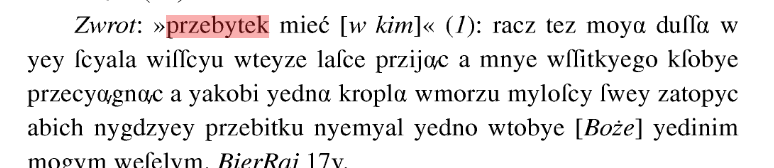
\includegraphics[width=1.00\hsize]{img/20_spxviw-31-42}
  \caption{SpXVIw t. 31 s. 42 --- \textit{Raj Duszny} s. 17v}
  \label{fig:RajDusznyS}
\end{figure}

\begin{figure}[h]
  \centering
  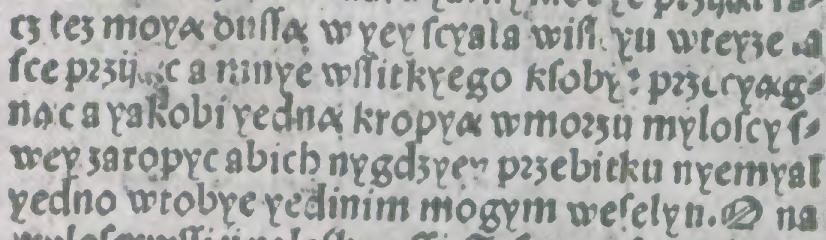
\includegraphics[width=1.00\hsize]{img/21_RajDusznyXVIIv}
  \caption{\textit{Raj Duszny} s. 17v}
  \label{fig:RajDuszny}
\end{figure}

W tekście widzimy m.in. literę alfa zwykłą i przekreśloną; jak
wspominałem o tym na liście dyskusyjnej standardu
(\url{http://unicode.org/mail-arch/unicode-ml/y2010-m08/0197.html}),
interpretowałbym ją jako \textit{LATIN SMALL LETTER ALPHA} (U+0251),
choć w większości fontów jej kształt nie jest satysfakcjonujący.


% [Raj duszny] Hortulus animae polonice. [Kraków, Florian Ungler i Wolfgang Lern, 1513] 8°
% http://www.wbc.poznan.pl/publication/418100
% @misc{_[Raj,
%  type={reprinty},
%  publisher={Wydawnictwo Poznańskie Studia Polonistyczne},
%  publisher={Biblioteka Uniwersytecka, Poznań},
%  title={[Raj duszny] Hortulus animae polonice. [Kraków, Florian Ungler i Wolfgang Lern, 1513] 8°},
%  language={pol},
%  keywords={raj, Hortulus, pierwsza drukowana książka polska, inkunabuł, starodruk},
% }

% {\it Zwrot}: »przebytek mieć [{\it w kim}]« ({\it 1}): racz tez moyα
% duſſα w yey ſcyala wiſſcyu wteyze laſce
% przijα\kv{-0.010}\kh{-0.130}{\raisebox{-0.7ex}[0pt][0pt]{{\small {\bf
% /}}}}\kv{0.010}c a mnye wſſitkyego kſobye
% przecyα\kv{-0.010}\kh{-0.130}{\raisebox{-0.7ex}[0pt][0pt]{{\small {\bf
% /}}}}\kv{0.010}gnα\kv{-0.010}\kh{-0.130}{\raisebox{-0.7ex}[0pt][0pt]{{\small
% {\bf /}}}}\kv{0.010}c a yakobi yednα kroplα wmorzu myloſcy ſwey
% zatopyc abich nygdzyey przebitku nyemyal yedno wtobye [{\it Boże}]
% yedinim mogym weſelym. {\it BierRaj} 17v.

% http://spxvi.edu.pl/instrukcja/

% Instrukcja redakcyjna
% Słownika polszczyzny XVI wieku

% Wersja elektroniczna oparta jest na Instrukcji redakcyjnej opracowanej
% przez Krystynę Wilczewską i wydanej do użytku wewnętrznego w 1976 r.


\section{Uwagi końcowe}
\label{sec:uwagi-kocowe}

Na witrynie konsorcjum Unicode znajdują się również notatki techniczne
(\textit{Unicode Technical Notes},
\url{http://www.unicode.org/notes/}), które nie są częścią standardu i
mają charakter czysto informacyjny. Autorami większości z nich są
współtwórcy standardu, ale nie jest to zasadą. Notatka nr 41
\textit{Church Slavonic Typography in Unicode} nasunęła mi myśl, że
można spróbować przygotować i zgłosić notatkę dotycząca
polszczyzny. Materiały do takiej notatki zacząłem gromadzić w
repozytorium
\url{https://github.com/jsbien/unicode4polish} (wcześniej
\url{https://bitbucket.org/jsbien/unicode4polish}),
częściowo w formie wiki
(\url{https://github.com/jsbien/unicode4polish/wiki}).
% https://bitbucket.org/jsbien/unicode4polish/wiki/Home}).
Okazało
się to jednak zbyt żmudne. Informacje bibliograficzne przeniosłem do
tzw. grupy systemu Zotero
(\url{https://www.zotero.org/groups/2196114/unicode_for_polish}),
niektóre inne informacje w miarę wolnego czasu umieszczałem w
odpowiednich hasłach Wikipedii,
por. np. \url{https://pl.wikipedia.org/wiki/Ƶ},
\url{https://pl.wikipedia.org/wiki/Ǫ}.

% https://pl.wikipedia.org/w/index.php?title=J&oldid=55014334

\textbf{Utworzone przeze mnie repozytoria nie są już przeze mnie
  rozwijane, ale będę się starał, aby były dostępne w Internecie przez
  rok od publikacji niniejszego artykułu [czyli do grudnia 2020 r.],
  potem zostaną zlikwidowane. Zainteresowane osoby proszone są więc o
  ich skopiowanie lub zgłoszenie się do mnie w celu przejęcia
  administracji repozytoriami. Do przejęcia lub współadministrowania
  dostępna jest również wspomniana wyżej grupa Zotero.}

% poprawić wikipedia
% poprawic note!:

\section{Podziękowania}
\label{sec:podzikowania}

Niniejszy artykuł został przygotowany --- jak wszystkie moje artykuły
-- za pomocą systemu \TeX{} (konkretnie \XeLaTeX). Na życzenie
Redakcji został on skonwertowany do formatu Worda (konkretnie do
akceptowanego przez Worda formatu \textsf{ODT}) za pomocą programu
\textsf{make4ht}; w dokonaniu konwersji pomógł mi istotnie autor
programu Michal Hoftich --- jestem mu za to bardzo wdzięczny.


\section*{Abstract}
\label{sec:abstract}

\textbf{The Unicode Standard and Polish language}

A short overview of the standard, together with the relevant tools and
resources, is presented from the historical Polish language
perspective. The notions of code space, code point, character,
combining sequence, graphemic cluster, variation selectors etc. are
presented or at least mentioned. A relatively new notion of
\textit{textel} is briefly discussed. The 15th and 16th century
treatises are used to illustrate some open problems. Various relevant
Internet resources are mentioned, including those created by the
author.


\printbibliography

\end{document}

\fontspec{CharisSILCompact}
\fontspec{Gentium Plus}

https://zalgo.org/#unZalgo_text

The Origin Of Zalgo

Zalgo is the creation of a Flash animator known as Dave Kelly. The
word “Zalgo” was often mentioned in Archies or Garfield comic strips
from the newspaper that used to denote something scary or full of
terror. It is also used to address a being who is often called as “he
who waits behind the wall”. The main purpose behind bringing the word
“Zalgo” was to represent the dark and demonic things with it.

łączliwość

https://lists.swift.org/pipermail/swift-evolution/Week-of-Mon-20160919/027245.html

https://manishearth.github.io/blog/2017/01/14/stop-ascribing-meaning-to-unicode-code-points/
https://eev.ee/blog/2015/09/12/dark-corners-of-unicode/

https://www.w3.org/2019/03/smufl13/specification/smufl-metadata.html
http://www.wbc.poznan.pl/publication/418100

2126;OHM SIGN                  ;Lu;0;L;03A9;;;;N;OHM;;;03C9;
03A9;GREEK CAPITAL LETTER OMEGA;Lu;0;L;    ;;;;N;;;;03C9;

%%% Local Variables:
%%% mode: latex
%%% ispell-local-dictionary: "polish"
%%% TeX-master: "JSB_tekstelePP"
%%% coding: utf-8-unix
%%% TeX-PDF-mode: t
%%% TeX-engine: xetex
%%% End:
